% Installation environnement de compilation et packages : 
% sudo apt-get install texlive-base texlive-lang-french texlive-latex-extra
% Compilation :
% depuis SRD/ :
% pdflatex src/SRD.tex 
% Si modification de l'index ou du glossaire, faire aussi :
% makeindex -s SRD.ist -t SRD.glg -o SRD.gls SRD.glo
% pdflatex src/SRD.tex 
% pdflatex src/SRD.tex 
% ou directement :
% make

\let\pagebreakORIG\pagebreak
\let\clearpageORIG\clearpage
\let\cleardoublepageORIG\cleardoublepage

\ifx \removepagebreak \undefined
	\newcommand{\removepagebreak}{\renewcommand{\pagebreak}{}\renewcommand{\clearpage}{}\renewcommand{\cleardoublepage}{}}
\fi

\ifx \restorepagebreak \undefined
	\newcommand{\restorepagebreak}{\renewcommand{\pagebreak}{\pagebreakORIG}\renewcommand{\clearpage}{\clearpageORIG}\renewcommand{\cleardoublepage}{\cleardoublepageORIG}}
\fi

\documentclass[a4paper,titlepage]{scrreprt}
\usepackage[utf8]{inputenc}
\usepackage[francais]{babel}
\usepackage[T1]{fontenc}
\usepackage[babel=true]{csquotes}
\usepackage{graphicx}
\usepackage{float}
%\usepackage{listings}
%\usepackage{underscore}
\usepackage[bookmarks=true]{hyperref}
\hypersetup{
    %bookmarks=false,    % show bookmarks bar?
    pdftitle={Quidditch Manager 2014 : Software Requirement Document},    % title
    pdfauthor={Groupe 4},                     % author
    pdfsubject={Software Requirement Document of the videogame Quidditch Manager 2014},                        % subject of the document
    pdfkeywords={SRD, Quidditch, Manager}, % list of keywords
    colorlinks=true,       % false: boxed links; true: colored links
    linkcolor=blue,       % color of internal links
    citecolor=black,       % color of links to bibliography
    filecolor=black,        % color of file links
    urlcolor=purple,        % color of external links
    linktoc=page            % only page is linked
}%
\usepackage{makeidx} %pour l'index
\usepackage{glossaries} %pour le glossaire
\usepackage{scrhack}
\usepackage{array} %tableaux
\usepackage{xcolor} % Required for specifying custom colors
\usepackage{fix-cm} % Allows increasing the font size of specific fonts beyond LaTeX default specifications
\usepackage{algorithm} %pseudo-code
\usepackage{algorithmic}
\usepackage{lscape} %paysage

%POUR LE TITRE :
\setlength{\oddsidemargin}{0mm} % Adjust margins to center the colored title box
\setlength{\evensidemargin}{0mm} % Margins on even pages - only necessary if adding more content to this template

\newcommand{\HRule}[1]{\hfill \rule{0.2\linewidth}{#1}} % Horizontal rule at the bottom of the page, adjust width here

\definecolor{grey}{rgb}{0.9,0.9,0.9} % Color of the box surrounding the title - these values can be changed to give the box a different color	

%Pour générer les fichiers pour makeIndex :
\makeindex
\makeglossaries

\begin{document}

\renewcommand{\glossaryname}{ }
\newglossaryentry{Quidditch}
{
  name=Quidditch,
  description={est un sport fictif issu de la saga
Harry Potter
créée par
J. K. Rowling.
Chaque équipe possède sept joueurs chevauchant des
balais volants. L'objectif étant de
marquer plus de points que l'adversaire en
marquant un maximum de buts et en
attrapant une balle magique, le
Vif d'or. Un match peut durer des mois et comporte des
risques mortels pour les joueurs}
}
\newglossaryentry{manager}
{
  name=manager,
  description={est l'utilisateur du programme, en charge de la gestion d'un club de Quidditch
  et de ses matchs}
}
\newglossaryentry{joueur}
{
  name=joueur,
  description={est un membre d'une équipe de Quidditch}
}
\newglossaryentry{match}
{
  name=match,
  description={est un affrontement de deux équipes de Quidditch sur un terrain}
}
\newglossaryentry{club}
{
  name=club,
  description={est un ensemble reprenant une équipe de Quidditch et son infrastructure}
}
\newglossaryentry{partie}
{
  name=partie,
  description={désigne la session de jeu que s'est créé l'utilisateur/Manager et qu'il peut gérer à sa guise. Il y a une partie par utilisateur}
}
\newglossaryentry{parcelle}
{
  name=parcelle,
  description={espace alloué à l'utilisateur où se trouvent ses bâtiments et son terrain de Quidditch}
}
\newglossaryentry{stade}
{
  name=stade,
  description={lieu sur l’espace alloué à un Manager où sont joués les matchs de Quidditch}
}
\newglossaryentry{terrain}
{
  name=terrain,
  description={espace à l'intérieur du stade où se déplacent les joueurs et les balles au cours d'un match}
}
\newglossaryentry{infirmerie}
{
  name=infirmerie,
  description={lieu où les joueurs du Managers sont soignés}
}
\newglossaryentry{centreentrainement}
{
  name=centre d’entrainement,
  description={lieu où le Manager peut faire s'entrainer ses joueurs}
}
\newglossaryentry{agencepublicite}
{
  name=agence de publicité,
  description={lieu où le Manager peut faire augmenter la popularité de ses joueurs}
}
\newglossaryentry{buvette}
{
  name=buvette,
  description={lieu où les supporters de l'équipe en déplacement pour un match qui ne se rendent pas sur place peuvent assister à une retransmission du match. Les consommations sont payantes et les bénéfices sont reversés au Manager}
}
\newglossaryentry{fanshop}
{
  name=fanshop,
  description={lieu où les supporters de l'équipe qui reçoit une équipe adverse pour un match peuvent acheter des produits dérivés}
}
\newglossaryentry{magasinbalais}
{
  name=magasin de balais,
  description={lieu où le Manager peut acheter/vendre des balais}
}
\newglossaryentry{centrerecrutement}
{
  name=centre de recrutement,
  description={lieu où le Manager peut acheter/vendre des joueurs}
}
\newglossaryentry{calendrier}
{
  name=calendrier,
  description={ensemble de rappels fixés dans le temps, le Manager est régulièrement rappelé à certaines actions (comme jouer un match) sur base de ce calendrier}
}

\newglossaryentry{evenement}
{
  name=événement,
  description={Action inscrite dans un calendrier qui rend possibles certains actions (jouer un match, sélectionner un joueur auparavant bloqué,...)}
}
\newglossaryentry{attrapeur}
{
  name=attrapeur,
  description={joueur dont la fonction au sein de l’équipe en cours de match est d’attraper le Vif d’Or}
}
\newglossaryentry{poursuiveur}
{
  name=poursuiveur,
  description={au nombre de 3 par équipe au cours d'un match, font des passes de Souafle entre eux et tentent de marquer des buts. Quand c'est l'équipe adverse qui a le souafle, ils essaient de le récupérer}
}
\newglossaryentry{batteur}
{
  name=batteur,
  description={au nombre de deux par équipe au cours d'un match. Un batteur frappe sur les Cognards et les envoie sur les joueurs adverses pour les blesser/déstabiliser}
}
\newglossaryentry{gardien}
{
  name=gardien,
  description={il n’y en a qu’un par équipe. Son rôle est d’empêcher les Poursuiveurs de l’équipe adverse de marquer des buts en interceptant leurs tirs}
}
\newglossaryentry{souafle}
{
  name=souafle,
  description={balle inerte unique manipulée pendant un match par les Poursuiveurs à travers des passes et des tentatives de tirs dans l’un des cercles d’or pour marquer un but}
}
\newglossaryentry{cognard}
{
  name=cognard,
  description={au nombre de deux. Plus petite que le Souafle. Balle magique qui essaie de frapper les joueurs pour les faire tomber de leur balais. Ces balles sont cognées par les batteurs pour les diriger vers les joueurs adverses}
}
\newglossaryentry{vifOr}
{
  name=vif d’Or,
  description={petite balle unique ayant sa propre volonté, qui se déplace aléatoirement et très rapidement dans les airs. Lorsqu’un Attrapeur attrape le Vif d’Or, la partie s’achève}
}

\renewcommand{\indexname}{4 Index}




\thispagestyle{empty} % Remove page numbering on this page

%----------------------------------------------------------------------------------------
%	TITLE SECTION
%----------------------------------------------------------------------------------------

\colorbox{grey}{
	\parbox[t]{1.0\linewidth}{
		\centering \fontsize{35pt}{80pt}\selectfont % The first argument for fontsize is the font size of the text and the second is the line spacing - you may need to play with these for your particular title
		\vspace*{0.7cm} % Space between the start of the title and the top of the grey box
		
		\hfill Quidditch Manager 2014 \\
		\hfill Software Requirements Document \\
		\hfill Projet d'année BA2 INFO - ULB\par
		
		\vspace*{0.7cm} % Space between the end of the title and the bottom of the grey box
	}
}

%----------------------------------------------------------------------------------------

\vfill % Space between the title box and author information

%----------------------------------------------------------------------------------------
%	AUTHOR NAME AND INFORMATION SECTION
%----------------------------------------------------------------------------------------

{\centering \large 
\hfill Groupe 4 : Manon Legrand, Hélène Plisnier, Audry Delestree, David Bertha \\
\hfill INFOF209 - Projet d'informatique - Quidditch Manager 2014 \\
\hfill Université Libre de Bruxelles \\
\hfill Version 3.0 \\

\HRule{1pt}} % Horizontal line, thickness changed here

%----------------------------------------------------------------------------------------

\clearpage % Whitespace to the end of the page

\tableofcontents
\chapter{Introduction}
\section{But du projet}
  % Texte (d’une demi-page approximativement) décrivant les tenants
  % et aboutissants du projet, et énumérant les différents types de
  % personnes qui vont bénéficier de la réalisation du projet.
  Le \gls{Quidditch}\index{Quidditch} \gls{manager}\index{manager} est un jeu multi-joueurs de gestion
  et de stratégie, se jouant en réseau.
  Un manager (l'utilisateur) gère son équipe de \gls{joueur}s, qu'il peut entrainer
  au travers des bâtiments construits sur la \index{parcelle}parcelle qui lui est attribuée. Certains de ces bâtiments permettent aussi de faire des achats et des ventes de balais ou de joueurs.
  Le but pour le manager est de déveloper son \gls{club} aussi bien au niveau commercial
  que sportif.
  À travers la construction et l'évolution de ses bâtiments, le manager ouvre et
  augmente des possibilités de gestion du club, notamment la possibilité
  d'améliorer les caractéristiques de ses joueurs, ces caractéristiques
  étant déterminantes dans le déroulement d'un match.
  Les différents managers sont périodiquement invités à s'affronter par
  ces \gls{match}s s'inscrivant dans un championnat, étalonné dans le temps. 
  
  Ces matchs se déroulent
  dans un stade propre à un des managers et apportent une entrée d'argent
  dûe notamment à la victoire d'une équipe mais aussi au nombre de tickets vendus.
  Au cours du match, les managers en présence choisissent à chaque tour de jeu
  des déplacements pour leurs différents joueurs. Il existe quatre fonction possible
  pour un joueur lors d'un match. Un joueur peut être un \gls{attrapeur}\index{joueur!attrapeur}, un \gls{batteur}\index{joueur!batteur}, un \gls{gardien}\index{joueur!gardien}
  ou un \gls{poursuiveur}\index{joueur!poursuiveur}.
  Chacun de ces rôles implique des actions possibles différentes au cours du match.
  Mais il est possible à chacun de se déplacer sur le terrain, celui-ci étant représenté par
  des hexagones (il y a donc 6 directions de déplacement possibles à partir d'une case).
  De plus, les joueurs se partagent le terrain avec les différentes balles du jeu, 
  qu'ils devront manipuler selon les règles pour emmener leur équipe vers la victoire,
  celle-ci étant déterminée lorsque le \gls{vifOr} est attrapé ou par abandon.


\section{Historique du document}
  % Tableau reprenant tous les changements effectués sur le
  % document. Chaque ligne de celui-ci contiendra les champs
  % suivants : numéro de version, auteur et date de la modification,
  % description des changements. Le tableau sera trié de manière
  % décroissante sur le numéro de version.
  \begin{tabular}{|c|c|c|c|}
    \hline
    Numéro de version & Auteur & Date de la modification & Description des changements \\
    \hline
    0.1 & David & 13/12/13 & Squelette du code \LaTeX \\
    0.2 & Hélène & 19/12/13 & Première ébauche de la section 2.1 \\
    0.3 & Manon & 20/12/13 & Section 2.1 finale \\
    0.4 & David & 20/12/13 & Sections 1,  2.2 et 2.3 \\
    0.5 & Manon & 20/12/13 & Section 3.1 \\
    0.5 & David & 20/12/13 & Section 3.2 \\
    0.6 & Audry & 20/12/13 & Section 3.3 \\
    0.7 & David & 20/12/13 & Glossaire et Index \\
    1.0 & Manon & 20/12/13 & Relecture et révision \\
    1.1 & Hélène & 07/02/14 & 1ère correction \\
    1.2 & Hélène & 20/02/14 & Communication réseau et Qt \\    
    1.3 & Audry & 21/02/14 & Nouveaux diagrammes de classes \\
    1.4 & Manon & 21/02/14 & Commentaires par rapport aux Use Case \\
    1.5 & Manon & 21/02/14 & Explications des diagrammes de classes \\
    1.6 & Audry & 21/02/14 & Nouveaux diagrammes de classes (2) \\
    1.7 & Manon & 21/02/14 & Modif de certains commentaires de diag \\
    2.0 & Manon & 21/02/14 & Jeu sur terminal et Echange de messages \\
    2.1 & David & 11/03/14 & Précisions de l'architecture réseau \\
    2.2 & Manon & 06/03/14 & Titre + Section 2.1 \\
    2.3 & Manon & 12/03/14 & Amélioration diags de classes \\
    2.4 & David & 12/03/14 & Diagramme de composants \\
    2.5 & David & 12/03/14 & Précisions sur le déroulement d'un match \\
    2.6 & David & 13/03/14 & Diagrammes pour la GUI \\
    2.7 & Hélène & 14/03/14 & Terminal graphique avec diagrammes détaillés\\
    \hline
  \end{tabular}


\section{Glossaire}
  % Définition des termes, des acronymes et des abréviations
  % utilisés dans le présent document.
  \removepagebreak
  \printglossaries
  \restorepagebreak
\chapter{Besoins de l'utilisateur}
  % Cette deuxième section reprend les services que le système doit
  % fournir aux utilisateurs, ainsi que les contraintes de
  % fonctionnement du système. Elle doit être complète et consistante,
  % et il faut qu’elle soit rédigée dans un langage spécialement
  % compréhensible pour le client, c’est-à-dire en évitant entre autres
  % tout terme ou détail techniques.
  
  
\section{Exigences fonctionnelles}
  % Ce type d’exigences sera décrit en utilisant des diagrammes use
  % case et en fournissant une description pour chacun d’entre eux
  % (comme vu au cours théorique et aux exercices).
  
  Les cas d'utilisation présentés ci-dessous décrivent les différentes actions proposées au client par le programme.

  \subsection{Cas d'utilisation 1: Démarrer le jeu}
  \begin{figure}[H]
    \center
    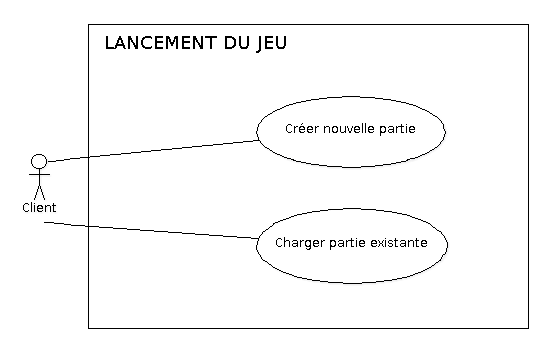
\includegraphics[scale=0.5]{uml/useCaseView/Lancementdujeu.png}
    \caption{Cas d'utilisation 1: Démarrer le jeu}
  \end{figure}  
    L'utilisateur démarre le jeu. Soit il a déjà commencé une \gls{partie}\index{partie}; dans ce cas, l'utilisateur s'identifie et reprend sa partie là où il l'avait laissée. \\
    Soit il ne possède pas encore de partie; le programme lui demande alors quelques informations d'identification. 
    Il se voit ensuite attribuer une équipe de 7 \gls{joueur}s médiocres et une \gls{parcelle}\index{parcelle}. 
    Au commencement, ce dernier est presque désert, composé uniquement d'un 
    \gls{stade}\index{bâtiment!Stade} de \gls{Quidditch}\index{Quidditch} et d'emplacements vides prévus pour accueillir les bâtiments.

    \subsubsection{Créer nouvelle partie}
      \begin{itemize}
        \item \textbf{Relations avec d'autres cas d'utilisation}  : Néant.
        \item \textbf{Pré-conditions} : Le client désire se créer une nouvelle partie.
        \item \textbf{Post-conditions} : Le client possède une partie.
        \item \textbf{Cas général} : Le client veut créer une nouvelle partie. Il devra alors rentrer toute une série d’informations concernant cette partie nécessaire à l’identification de cette partie et au bon fonctionnement du jeu (nom du \index{manager}manager, nom de l’équipe, mot de passe, etc.)
        \item \textbf{Cas exceptionnels} :
          \begin{itemize}
            \item Un manager avec le nom indiqué par le client existe déjà. Le programme le signale au client qui doit de nouveau choisir ce qu'il veut faire.
          \end{itemize}
      \end{itemize}

    \subsubsection{Charger partie existante}
      \begin{itemize}
        \item \textbf{Relations avec d'autres cas d'utilisation}  : Néant.
        \item \textbf{Pré-conditions} : Il faut qu’il existe déjà une partie à laquelle créée par ce client.
        \item \textbf{Post-conditions} : Le client a accès à sa partie.
        \item \textbf{Cas général} : Le client souhaite continuer une partie déjà entamée et rentre le nom de la partie ainsi que le mot de passe pour récupérer les informations concernant cette partie.
        \item \textbf{Cas exceptionnels} :
          \begin{itemize}
      \item L’identification de la partie a échoué (mauvais nom ou mot de passe). Le programme le signale au client qui doit de nouveau choisir ce qu'il veut faire.
          \end{itemize}
      \end{itemize}

  \subsection{Cas d'utilisation 2: Gestion de l'équipe}
  \begin{figure}[H]
    \center
    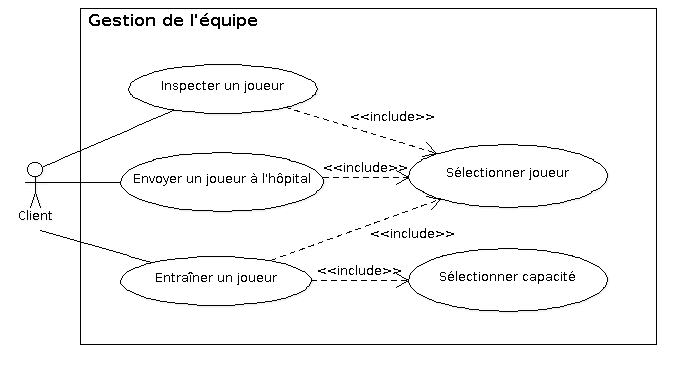
\includegraphics[scale=0.5]{uml/useCaseView/GestionEquipe.png}
    \caption{Cas d'utilisation 2: Gestion de l'équipe}
  \end{figure}  
    Une fois que l'utilisateur a rejoint sa \gls{partie}\index{partie} ou en a créé une nouvelle, il peut gérer son équipe. Le manager peut alors au choix se renseigner sur ses joueurs, et donc voir les capacitiés de ce dernier, l'avancement de ses entraînements, etc. Il peut également envoyer un joueur au centre d'entraînement ou à l'hôpital.

    \subsubsection{Inspecter un joueur}
      \begin{itemize}
        \item \textbf{Relations avec d'autres cas d'utilisation}  : Inclut Sélectionner joueur.
        \item \textbf{Pré-conditions} : Néant.
        \item \textbf{Post-conditions} : Une \"fiche d'identité\" du joueur est affichée.
        \item \textbf{Cas général} : Le client/manager souhaite se renseigner sur un de ses joueurs. Il sélectionne le joueur concerné pour avoir les informations sur ce dernier. Ces informations sont : les capacités, l'avancement des entraînements par capacité, une indication quant au blocage (entraînement/hôpital/enchères) éventuel du joueur, les informations sur le balai du joueur et une estimation de la valeur du joueur.
        \item \textbf{Cas exceptionnels} : Néant.
      \end{itemize}

    \subsubsection{Envoyer un joueur à l'hôpital}
      \begin{itemize}
        \item \textbf{Relations avec d'autres cas d'utilisation}  : Inclut Sélectionner joueur.
        \item \textbf{Pré-conditions} : Le joueur sélectionné n'est pas bloqué par un entraînement, un séjour à l'hôpital ou une enchère et le client possède suffisamment de points d'action pour envoyer son joueur à l'hôpital.
        \item \textbf{Post-conditions} : Le joueur est soigné mais bloqué pour une durée qui dépend du niveau de l'hôpital.
        \item \textbf{Cas général} : Le client souhaite soigner un joueur qui a été blessé au cours d'un match et l'envoie donc à l'hôpital pour que lui soient procurés les soins requis.
        \item \textbf{Cas exceptionnels} : Néant.
      \end{itemize}

    \subsubsection{Entraîner un joueur}
      \begin{itemize}
        \item \textbf{Relations avec d'autres cas d'utilisation}  : Inclut Sélectionner joueur et Sélectionner capacité.
        \item \textbf{Pré-conditions} : Le joueur sélectionné n'est pas bloqué par un entraînement, un séjour à l'hôpital ou une enchère et le client possède suffisamment de points d'action pour que son joueur commence un entraînement.
        \item \textbf{Post-conditions} : L'avancement de l'entraînement de la capacité concernée du joueur choisi est incrémenté, si l'avancement devient complet, c'est-à-dire si le nombre de sessions d'entraînement requis pour passer au niveau supérieur est atteint, la capacité est incrémentée et l'avancement est réinitialisé.
        \item \textbf{Cas général} : Le client souhaite entraîner un joueur pour le faire progresser dans une capacité.
        \item \textbf{Cas exceptionnels} : Néant.
      \end{itemize}

    \subsubsection{Sélectionner joueur}
      \begin{itemize}
        \item \textbf{Relations avec d'autres cas d'utilisation}  : Est inclus dans Inspecter joueur, Envoyer un joueur à l'hôpital et Entraîner joueur.
        \item \textbf{Pré-conditions} : Néant.
        \item \textbf{Post-conditions} : Le joueur est sélectionné.
        \item \textbf{Cas général} : Le client choisit le joueur qui l'intéresse pour l'inspection, l'envoi à l'hôpital ou l'entraînement.
        \item \textbf{Cas exceptionnels} : Néant.
      \end{itemize}

    \subsubsection{Sélectionner capacité}
      \begin{itemize}
        \item \textbf{Relations avec d'autres cas d'utilisation}  : Est inclus dans Entraîner joueur.
        \item \textbf{Pré-conditions} : Néant.
        \item \textbf{Post-conditions} : La capacité est sélectionnée.
        \item \textbf{Cas général} : Le client choisit la capacité qu'il veut entraîner pour le joueur concerné.
        \item \textbf{Cas exceptionnels} : Néant.
      \end{itemize}

 \subsection{Cas d'utilisation 3: Gestion du domaine}
  \begin{figure}[H]
    \center
    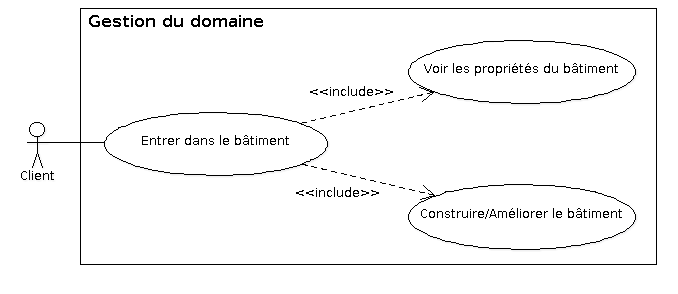
\includegraphics[scale=0.5]{uml/useCaseView/GestionDomaine.png}
    \caption{Cas d'utilisation 3: Gestion du domaine}
  \end{figure}  
    Une fois que l'utilisateur a rejoint sa \gls{partie}\index{partie} ou en a créé une nouvelle, il peut gérer son domaine. Au commencement du jeu, ce domaine comprend un stade de petite taille, des infrastructures médiocres pour les entraînements et les soins à procurer aux joueurs, qui deviendront un beau centre d'entraînement et un hôpital à la pointe de la technologie, et également d'emplacements pour un fan shop et un centre de promotion (pour gagner des points d'action). Le client peut donc entamer des projets de construction et d'améliorer de bâtiments pour que ces derniers soient plus performants ou plus lucratifs.

    \subsubsection{Entrer dans le bâtiment}
      \begin{itemize}
        \item \textbf{Relations avec d'autres cas d'utilisation}  : Inclut Voir les propriétés du bâtiment et Construire/Améliorer le bâtiment.
        \item \textbf{Pré-conditions} : Néant.
        \item \textbf{Post-conditions} : Le client est dans le bâtiment.
        \item \textbf{Cas général} : Le client \"rentre\" dans le bâtiment et a la possibilité de lancer un projet de construction ou d'obtenir les informations concernant ce bâtiment.
        \item \textbf{Cas exceptionnels} : Néant.
      \end{itemize}

    \subsubsection{Voir les propriétés du bâtiment}
      \begin{itemize}
        \item \textbf{Relations avec d'autres cas d'utilisation}  : Est inclus dans Entrer dans le bâtiment.
        \item \textbf{Pré-conditions} : Néant.
        \item \textbf{Post-conditions} : Les informations du bâtiment s'affichent.
        \item \textbf{Cas général} : Le client souhaite avoir des renseignements sur le bâtiment dans lequel il est entré, s'affichent alors le niveau du bâtiment, le montant à payer et le nombre de points d'action nécessaires pour passer au niveau suivant et les caractéristiques particulières propres au bâtiment (comme par exemple le nombre de places s'il s'agit du stade).
        \item \textbf{Cas exceptionnels} : Néant.
      \end{itemize}

    \subsubsection{Construire/Améliorer le bâtiment}
      \begin{itemize}
        \item \textbf{Relations avec d'autres cas d'utilisation}  : Est inclus dans Entrer dans le bâtiment.
        \item \textbf{Pré-conditions} : Le client doit posséder suffisamment d'argent et de points d'action pour lancer le projet de construction ou d'amélioration. Il ne doit pas y avoir non plus un projet en cours sur ce bâtiment.
        \item \textbf{Post-conditions} : Le bâtiment est en projet pour une durée déterminée par son niveau. A la fin de ce laps de temps, le niveau du bâtiment sera incrémenté.
        \item \textbf{Cas général} : Le client souhaite améliorer le bâtiment dans lequel il est entré et est prêt à dépenser de l'argent et des points d'action pour ce faire.
        \item \textbf{Cas exceptionnels} : Néant.
      \end{itemize}


  \subsection{Cas d'utilisation 4: Enchères}
  \begin{figure}[H]
    \center
    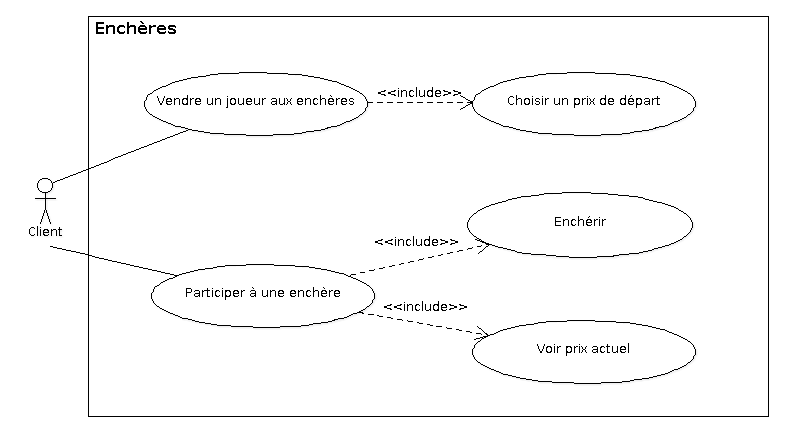
\includegraphics[scale=0.5]{uml/useCaseView/Encheres.png}
    \caption{Cas d'utilisation 4: Gestion de l'équipe}
  \end{figure}  
    L'utilisateur n'étant pas obligé de se coltiner à vie son équipe de bras cassés, il peut acheter des joueurs mis en enchères par d'autres utilisateurs, ou même se débarasser des siens en les mettant en vente. Pour participer à une enchère, l'utilisateur doit faire une première offre, il est alors inscrit au tour suivant. A chaque enchère faite par un participant, le prix d'achat augmente de 10\% du prix de départ. La vente se déroule par tour. A chacun de ces tours, les participants peuvent choisir d'enchérir ou non. S'ils enchérissent, ils sont inscrits pour le tour suivant, sinon, ils quittent la vente. Lorsqu'il n'y a qu'un seul participant qui enchérit au cours d'un tour, c'est lui qui remporte l'enchère. Si par contre aucun participant n'a enchéri avant la fin du tour actuel, c'est celui qui a enchéri en dernier au tour précédent qui remporte l'enchère. La transaction peut alors se faire. 

    \subsubsection{Vendre un joueur aux enchères}
      \begin{itemize}
        \item \textbf{Relations avec d'autres cas d'utilisation}  : Inclut Choisir un prix de départ.
        \item \textbf{Pré-conditions} : Le joueur que le client souhaite vendre n'est pas bloqué par un entraînement ou un séjour à l'hôpital.
        \item \textbf{Post-conditions} : Le joueur mis en vente est bloqué pour toute la durée de l'enchère.
        \item \textbf{Cas général} : Le client souhaite vendre un joueur pour se débarasser de lui et gagner de l'argent.
        \item \textbf{Cas exceptionnels} :
          \begin{itemize}
            \item Si la vente du joueur réussit et que le client a désormais moins de 7 joueurs dans son équipe, il ne pourra plus faire de matches tant qu'il n'aura pas racheté des joueurs pour compléter son équipe.
          \end{itemize}
      \end{itemize}

    \subsubsection{Participer à une enchère}
      \begin{itemize}
        \item \textbf{Relations avec d'autres cas d'utilisation}  : Inclut Enchérir et Voir prix actuel.
        \item \textbf{Pré-conditions} : Néant.
        \item \textbf{Post-conditions} : Le client ne peut rien faire d'autre tant qu'il participe à l'enchère.
        \item \textbf{Cas général} : Le client est intéressé par le joueur et participe aux enchères. Il s'inscrit en faisant une première enchère.
        \item \textbf{Cas exceptionnels} :
          \begin{itemize}
            \item Si le client participe à une enchère qu'il a lui-même créée, il est considéré comme un participant lambda et peut donc remporter l'enchère. S'il gagne, il se versera l'argent à lui-même, et achètera son propre joueur, ce qui est une perte de temps.
          \end{itemize}
      \end{itemize}

    \subsubsection{Choisir un prix de départ}
      \begin{itemize}
        \item \textbf{Relations avec d'autres cas d'utilisation}  : Est inclus dans Vendre un joueur aux enchères.
        \item \textbf{Pré-conditions} : Néant.
        \item \textbf{Post-conditions} : Le prix de départ déterminera le prix réel de vente puisque chaque enchère fait augmenter le prix de 10\% du prix de départ.
        \item \textbf{Cas général} : Le client choisit le prix de départ de l'enchère. Il peut ne pas respecter le montant estimé du joueur, mais c'est à ses risques et périls. Un prix de départ trop cher pourrait rebuter les acheteurs, et un prix de départ trop faible pourrait représenter une perte économique.
        \item \textbf{Cas exceptionnels} : Néant.
      \end{itemize}

    \subsubsection{Enchérir}
      \begin{itemize}
        \item \textbf{Relations avec d'autres cas d'utilisation}  : Est inclus dans Participer à une enchère.
        \item \textbf{Pré-conditions} : Le client n'a pas encore enchéri pendant le tour actuel.
        \item \textbf{Post-conditions} : Le client est inscrit pour le prochain tour de l'enchère.
        \item \textbf{Cas général} : Le client est toujours intéressé par le joueur et enchérit car il veut remporter l'enchère.
        \item \textbf{Cas exceptionnels} : Néant.
      \end{itemize}

    \subsubsection{Voir prix actuel}
      \begin{itemize}
        \item \textbf{Relations avec d'autres cas d'utilisation}  : Est inclus dans Participer à une enchère.
        \item \textbf{Pré-conditions} : Néant.
        \item \textbf{Post-conditions} : Le prix actuel de l'enchère est affiché.
        \item \textbf{Cas général} : Le client souhaite voir à combien s'élève le montant qu'il devrait débourser pour acheter le joueur s'il remportait l'enchère maintenant.
        \item \textbf{Cas exceptionnels} : Néant.
      \end{itemize}


  \subsection{Cas d'utilisation 5: Matches}
  \begin{figure}[H]
    \center
    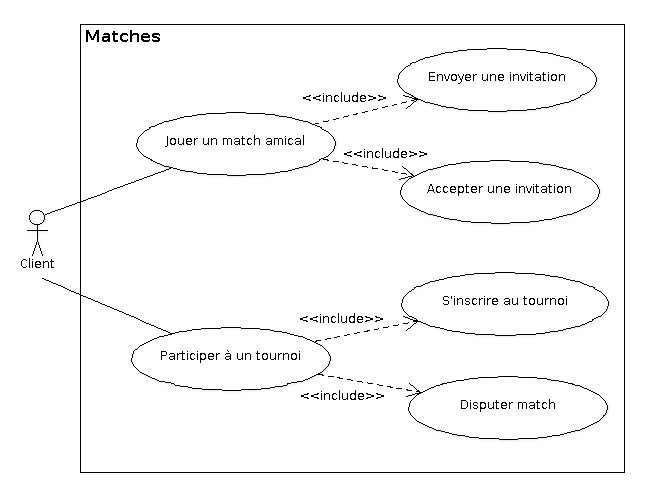
\includegraphics[scale=0.5]{uml/useCaseView/Matches.png}
    \caption{Cas d'utilisation 5: Matches}
  \end{figure}  
    L'utilisateur a la possibilité de mettre ses joueurs en action au cours de vrais matches de Quidditch. Pour cela, il peut soit s'inscrire à un tournoi, soit proposer un match amical à un autre utilisateur connecté. Dans le cadre d'un tournoi, les tours de matchs démarrent une fois que le bon nombre d'inscrits est atteint. L'utilisateur qui jouera le mieux, ou qui sera le plus chanceux, remportera le tournoi et les récompenses qui vont avec. Gagner un match amical offre également des avantages mais qui sont, bien entendu, moins conséquents.

    \subsubsection{Jouer un match amical}
      \begin{itemize}
        \item \textbf{Relations avec d'autres cas d'utilisation}  : Inclut Envoyer une invitation et Accepter une invitation.
        \item \textbf{Pré-conditions} : Néant.
        \item \textbf{Post-conditions} : Si le client remporte le match, ou qu'il y a match nul, il recevra une certaine somme d'argent en récompense.
        \item \textbf{Cas général} : Le client a envoyé une invitation qui a été acceptée par l'adversaire ou a accepté une invitation qui lui a été envoyée et va donc affronter un autre utilisateur. Le match commencera quand les deux utilisateurs auront désigné les joueurs et leur poste.
        \item \textbf{Cas exceptionnels} : Néant.
      \end{itemize}

    \subsubsection{Participer à un tournoi}
      \begin{itemize}
        \item \textbf{Relations avec d'autres cas d'utilisation}  : Inclut S'inscrire au tournoi et Disputer match.
        \item \textbf{Pré-conditions} : Néant.
        \item \textbf{Post-conditions} : A chaque match gagné lors du tournoi, le client reçoit de l'argent en récompense.
        \item \textbf{Cas général} : Le client s'est inscrit à un tournoi (créé par l'administrateur). Lorsqu'il y a suffisament d'inscrits, le tournoi démarre tous les matchs du premier tour. Dès qu'un tour est terminé, le tour suivant
        commence (avec les joueurs ayant gagné leur match du tour précédent), jusqu'à ce qu'il n'y ait qu'un gagnant.
        \item \textbf{Cas exceptionnels} : Néant.
      \end{itemize}

    \subsubsection{Envoyer une invitation}
      \begin{itemize}
        \item \textbf{Relations avec d'autres cas d'utilisation}  : Est inclus dans Jouer un match amical.
        \item \textbf{Pré-conditions} : Le client possède suffisamment de points d'action pour envoyer une demande et il possède au moins 7 joueurs non bloqués dans son équipe.
        \item \textbf{Post-conditions} : Le client ne peut rien faire tant qu'il attend la réponse de l'autre utilisateur. Si l'adversaire accepte, les points d'action sont retirés et le match commence, sinon le client revient à sa session de jeu et aucun point d'action ne lui sera retiré.
        \item \textbf{Cas général} : Le client a accès à la liste des utilisateurs connectés et choisit celui contre qui il a envie de disputer un match amical.
        \item \textbf{Cas exceptionnels} : Néant.
      \end{itemize}

    \subsubsection{Accepter une invitation}
      \begin{itemize}
        \item \textbf{Relations avec d'autres cas d'utilisation}  : Est inclus dans Jouer un match amical.
        \item \textbf{Pré-conditions} : Le client a au moins 7 joueurs non bloqués dans son équipe.
        \item \textbf{Post-conditions} : Le match commence.
        \item \textbf{Cas général} : Le client a reçu une invitation d'un autre utilisateur connecté qui souhaite l'affronter au cours d'un match amical.
        \item \textbf{Cas exceptionnels} : Néant.
      \end{itemize}

    \subsubsection{S'inscrire au tournoi}
      \begin{itemize}
        \item \textbf{Relations avec d'autres cas d'utilisation}  : Est inclus dans Participer à un tournoi.
        \item \textbf{Pré-conditions} : Néant.
        \item \textbf{Post-conditions} : Le client est inscrit à ce tournoi et ne pourra donc pas s'inscrire à un autre tournoi.
        \item \textbf{Cas général} : Le client a accès à la liste des tournois pour lesquels il manque encore des participants et a la possibilité de s'inscrire à l'un deux.
        \item \textbf{Cas exceptionnels} : Néant.
      \end{itemize}

        \subsubsection{Disputer match}
      \begin{itemize}
        \item \textbf{Relations avec d'autres cas d'utilisation}  : Est inclus dans Participer à un tournoi.
        \item \textbf{Pré-conditions} : Le client a au moins 7 joueurs non bloqués dans son équipe.
        \item \textbf{Post-conditions} : Si le client remporte le match, il est qualifié pour le tour d'après et gagne de l'argent.
        \item \textbf{Cas général} : Le jour de l'affrontement dans le cadre du tournoi est arrivé et le client va jouer son match contre son adversaire.
        \item \textbf{Cas exceptionnels} :
          \begin{itemize}
            \item Le match était le dernier du tour du tournoi. Le tour suivant commence alors.
            \item Si le résultat est un match nul, le gagnant est alors celui qui a proposé le match nul.
          \end{itemize}
      \end{itemize}


  \subsection{Cas d'utilisation 6: Tour d'un match}
  \begin{figure}[H]
    \center
    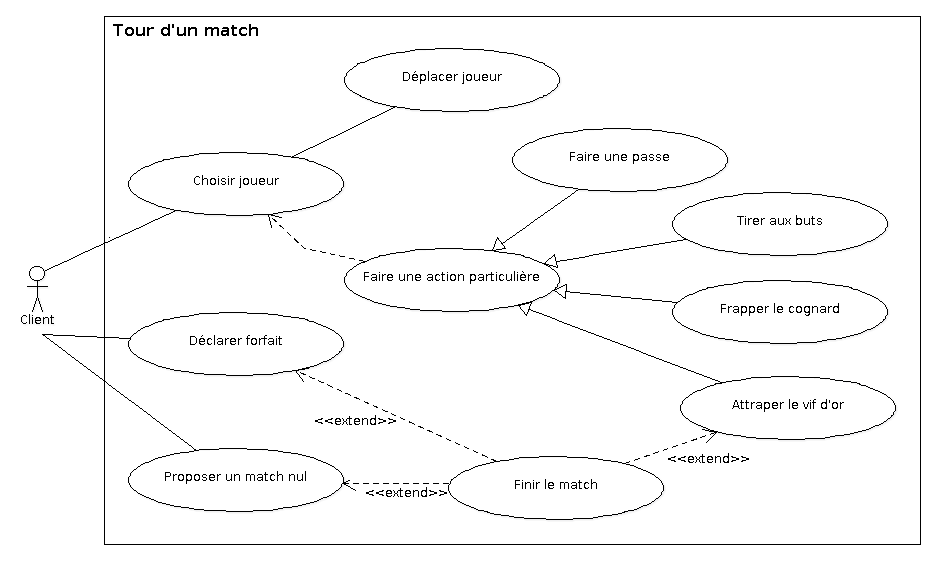
\includegraphics[scale=0.5]{uml/useCaseView/TourMatch.png}
    \caption{Cas d'utilisation 6: Tour d'un match}
  \end{figure}  
    Les matches se jouent au tour par tour. A chaque tour, les clients qui s'affrontent sont invités à indiquer les actions (déplacement ou action particulière) à faire pour chacun de leur joueur. %Ils ont un temps limité pour indiquer ces actions. Une fois le temps écoulé, seules les indications déjà enregistrées seront prises en compte.

    \subsubsection{Choisir joueur}
      \begin{itemize}
        \item \textbf{Relations avec d'autres cas d'utilisation}  : Précède Déplacer joueur et Faire une action particulière (ce use case dépendant de celui-ci : en effet, les actions possibles changent en fonction du joueur choisi).
        \item \textbf{Pré-conditions} : Le client n'a pas déjà choisi quoi faire pour ce joueur.
        \item \textbf{Post-conditions} : Le client ne pourra plus choisir quoi faire pour ce joueur.
        \item \textbf{Cas général} : Le client va, pour chaque tour, indiquer à chacun de ses joueurs ce qu'il doit faire; se déplacer ou effectuer une action particulière dépendant du joueur (faire une passe, etc.). Le joueur peut également rester sur place et ne rien faire (c'est en quelque sorte un déplacement de longueur 0).
        \item \textbf{Cas exceptionnels} : Néant.
      \end{itemize}

    \subsubsection{Déplacer joueur}
      \begin{itemize}
        \item \textbf{Relations avec d'autres cas d'utilisation}  : Lié à Choisir joueur
        \item \textbf{Pré-conditions} : Néant.
        \item \textbf{Post-conditions} : Le joueur sélectionné a été déplacé ou est resté sur place.
        \item \textbf{Cas général} : Le client sélectionne un joueur et choisit où celui-ci doit se déplacer sur le terrain\index{terrain} ou le laisse sur place. Le client est informé de l’ensemble des destinations possibles pour le joueur sélectionné.
        \item \textbf{Cas exceptionnels} : 
        \begin{itemize}
            \item Le client ne choisi aucune direction pour le joueur sélectionné. Le joueur reste donc sur place.
          \end{itemize}
      \end{itemize}

    \subsubsection{Faire une action particulière}
      \begin{itemize}
        \item \textbf{Relations avec d'autres cas d'utilisation}  : Dépend de Choisir joueur. Généralise Faire une passe, Tirer aux buts, Frapper le cognard et Attraper le vif d'or.
        \item \textbf{Pré-conditions} : Néant.
        \item \textbf{Post-conditions} : Le joueur a une action particulière à accomplir, ses chances de réussir dépendent de ses capacités.
        \item \textbf{Cas général} : Le client choisit le joueur et l’action que celui-ci doit réaliser. Cette action dépend du poste du joueur.
        \item \textbf{Cas exceptionnels} : Néant.
      \end{itemize}

    \subsubsection{Faire une passe}
      \begin{itemize}
        \item \textbf{Relations avec d'autres cas d'utilisation}  : Spécialise Faire une action particulière.
        \item \textbf{Pré-conditions} : Le joueur qui va faire la passe doit tenir le \gls{souafle}\index{balle!souafle} et doit être un \gls{poursuiveur}s \index{joueur!poursuiveur} ou un \gls{gardien}s \index{joueur!gardien}.
        \item \textbf{Post-conditions} : Que la passe soit réussie ou ratée, le joueur ne possèdera plus le souafle.
        \item \textbf{Cas général} : Le client choisit l’endroit de destination de la passe. Les endroits possibles dépendent des compétences du joueur qui a le souafle. %Attraper le souafle suite à une passe ou l’intercepter (passe adverse) se fait de façon automatique par un poursuiveur se trouvant sur la trajectoire de la passe.
        \item \textbf{Cas exceptionnels} :
        \begin{itemize}
            %\item Le joueur est heurté par un \gls{cognard}\index{balle!cognard}. La passe échoue. 
            \item La balle entre en collision avec une autre balle ou un joueur. Son déplacement s'arrête.
        \end{itemize}
      \end{itemize}

     \subsubsection{Tirer aux buts}
      \begin{itemize}
        \item \textbf{Relations avec d'autres cas d'utilisation}  : Spécialise Faire une action particulière.
        \item \textbf{Pré-conditions} : Le poursuiveur qui veut tirer doit tenir le souafle et se trouver dans l’alignement d’un des buts. 
        \item \textbf{Post-conditions} : Qu’il y ait but ou non, le joueur ne tiendra plus le souafle.
        \item \textbf{Cas général} : Le client essaie de marquer un but en indiquant au poursuiveur détenant le souafle vers quel but il doit tirer.  Si le tir est réussi, l'équipe qui vient de marquer gagne 10 points. %Intercepter le souafle se fait automatiquement par le \gls{gardien}\index{joueur!gardien} ou les \gls{poursuiveur}s \index{joueur!poursuiveur} adverses s’ils se trouvent sur la trajectoire du souafle.
         \item \textbf{Cas exceptionnels} :
           \begin{itemize}
%         \item Le poursuiveur qui s'apprête à tirer est heurté par un \gls{cognard}\index{balle!cognard}. Le tir au but échoue. 
            \item La balle entre en collision avec une autre balle ou un joueur. Son déplacement s'arrête.
           \end{itemize}
      \end{itemize}

    \subsubsection{Frapper le cognard}
      \begin{itemize}
        \item \textbf{Relations avec d'autres cas d'utilisation}  : Spécialise Faire une action particulière
        \item \textbf{Pré-conditions} : Le joueur qui va essayer de frapper un \gls{cognard}\index{balle!cognard} doit être un batteur\index{joueur!batteur} et doit se situer près du cognard.
        \item \textbf{Post-conditions} : Le cognard est projeté dans la direction voulue.
        \item \textbf{Cas général} : Le code client indique dans quelle direction le batteur doit frapper le cognard.
        \item \textbf{Cas exceptionnels} :
          \begin{itemize}
        \item Le batteur rate son coup. Rien ne se passe.%Le cognard heurte le joueur.
          \end{itemize}
      \end{itemize}

    \subsubsection{Attraper le vif d'or}
      \begin{itemize}
        \item \textbf{Relations avec d'autres cas d'utilisation}  : Spécialise Faire une action particulière et est étendu par Finir le match
        \item \textbf{Pré-conditions} : Un des \gls{attrapeur}s \index{joueur!attrapeur} a repéré le \gls{vifOr}.
        \item \textbf{Post-conditions} : Si l'attrapeur réussit son coup, le match est terminé. S'il échoue, le match continue.
        \item \textbf{Cas général} : Un des attrapeurs est arrivé à proximité du vif d'or. Il essaiera alors de l’attraper (la réussite de l’action dépend des qualités de l’attrapeur et de sa distance par rapport au vif d’or). S’il réussit à l’attraper, son équipe gagne 150 points et le match est terminé.
        \item \textbf{Cas exceptionnels} :
         \begin{itemize}
            %\item L'attrapeur est heurté par un cognard. Le vif d'or reste libre.
            \item L'attrapeur échoue. Le vif d'or reste libre.    
        \end{itemize}
      \end{itemize}

    \subsubsection{Déclarer forfait}
      \begin{itemize}
        \item \textbf{Relations avec d'autres cas d'utilisation}  : Est étendu par Finir le match.
        \item \textbf{Pré-conditions} : L'action se déroule au cours d'un match.
        \item \textbf{Post-conditions} : Le match est terminé. Le client qui n'a pas déclaré forfait a gagné.
        \item \textbf{Cas général} : Un des client souhaite mettre fin au match en déclarant forfait (équivaut à une défaite 150-0, peu importe le score lorsqu’il déclare forfait).
        \item \textbf{Cas exceptionnels} :
          \begin{itemize}
            \item Si un client se déconnecte au cours d’un match, on considérera qu’il a déclaré forfait.
          \end{itemize}
      \end{itemize}

    \subsubsection{Proposer un match nul}
      \begin{itemize}
        \item \textbf{Relations avec d'autres cas d'utilisation}  : Est étendu par Finir le match.
        \item \textbf{Pré-conditions} : L'action se déroule au cours d'un match.
        \item \textbf{Post-conditions} : Si l'adversaire accepte la proposition, le match sera terminé, sinon le match continue.
        \item \textbf{Cas général} : Un des client souhaite mettre fin au match en proposant un match nul à l'adversaire. %Un match nul a l'avantage que chacun des clients recevra une petite récompense.
        \item \textbf{Cas exceptionnels} :
          \begin{itemize}
            \item Il s'agit d'un match de tournoi. Celui ayant demandé la fin du match est considéré comme perdant.
          \end{itemize}
      \end{itemize}

    \subsubsection{Finir le match}
      \begin{itemize}
        \item \textbf{Relations avec d'autres cas d'utilisation}  : Etend Attraper le vif d'or, Déclarer forfait et proposer un match nul.
        \item \textbf{Pré-conditions} : Néant.
        \item \textbf{Post-conditions} : Il y a un club gagnant et un club perdant ou deux ex-aequos.
        \item \textbf{Cas général} : Le match va se terminer, le score est figé et les résultats vont déterminer ce que va gagner ou perdre (argent, fans) chaque client.
        \item \textbf{Cas exceptionnels} :
          \begin{itemize}
%            \item Le match se finit parce que les deux clients qui s’affrontent se sont déconnectés et n’ont pas joué le match jusqu’au bout. Le match est considéré comme annulé.
%            \item Si les 7 joueurs d'une même équipe sont blessés et ne peuvent continuer à jouer, l'équipe adverse gagnera le match.
            \item Un des clubs a déclaré forfait. L'autre club est gagnant.
          \end{itemize}
      \end{itemize}


  \subsection{Cas d'utilisation 7: Points d'action}
  \begin{figure}[H]
    \center
    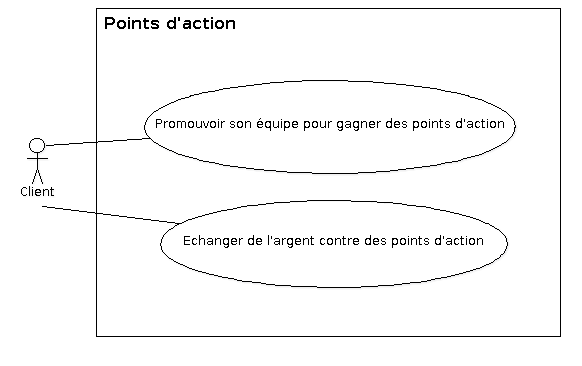
\includegraphics[scale=0.5]{uml/useCaseView/PointsAction.png}
    \caption{Cas d'utilisation 7: Points d'action}
  \end{figure}  
    L'utilisateur possède un certain nombre de points d'action qui limite ce qu'il peut faire. En effet, chaque action de gestion, qu'elle ait un coût financier ou non, ne peut être exécutée que si le client possède suffisamment de points d'action. Puisque ces points sont vite dépensés, il faut bien que l'utilisateur puisse en récupérer.

    \subsubsection{Promouvoir son équipe pour gagner des points d'action}
      \begin{itemize}
        \item \textbf{Relations avec d'autres cas d'utilisation}  : Néant.
        \item \textbf{Pré-conditions} : Néant.
        \item \textbf{Post-conditions} : Le client ne peut rien faire d'autre tant qu'il n'aura pas quitté sa campagne de promotion. Une fois celle-ci terminée (choix du client), il gagnera des points d'action.
        \item \textbf{Cas général} : Le client veut récupérer gratuitement des points d'action et va donc promouvoir son équipe. Il s'agit d'une attente active : au plus longtemps il attend, au plus de points d'action il pourra récupérer. Ce nombre dépend également du niveau du centre de promotion.
        \item \textbf{Cas exceptionnels} :
          \begin{itemize}
            \item Le client se déconnecte en pleine campagne. Il n'aura gagné aucun point d'action.
          \end{itemize}
      \end{itemize}

    \subsubsection{Echanger de l'argent contre des points d'action}
      \begin{itemize}
        \item \textbf{Relations avec d'autres cas d'utilisation}  : Néant.
        \item \textbf{Pré-conditions} : Le client doit posséder suffisamment d'argent.
        \item \textbf{Post-conditions} : De l'argent est retiré au client et des points d'action lui sont redistribués.
        \item \textbf{Cas général} : Le client souhaite gagner immédiatement des points d'action et est prêt à mettre la main au portefeuille pour ce faire. Le taux de change or-point d'action est préfixé et est le même pour tous les utilisateurs.
        \item \textbf{Cas exceptionnels} : Néant.
      \end{itemize}


  \subsection{Cas d'utilisation 8: Session de l'administrateur}
  \begin{figure}[H]
    \center
    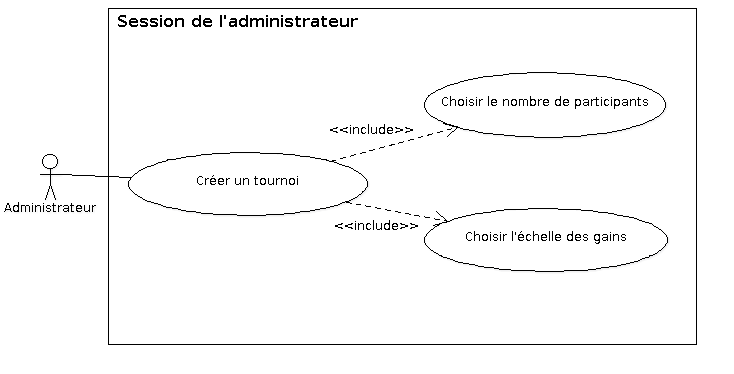
\includegraphics[scale=0.5]{uml/useCaseView/SessionAdmin.png}
    \caption{Cas d'utilisation 8: Session de l'administrateur}
  \end{figure}  
    L'administrateur est un utilisateur particulier qui n'a pas de session de jeu comme les autres mais qui peut créer des tournois.

    \subsubsection{Créer un tournoi}
      \begin{itemize}
        \item \textbf{Relations avec d'autres cas d'utilisation}  : Inclut Choisir le nombre de participants et Choisir l'échelle des gains.
        \item \textbf{Pré-conditions} : Néant.
        \item \textbf{Post-conditions} : Le tournoi est créé.
        \item \textbf{Cas général} : L'administrateur décide de créer un tournoi pour que les utilisateurs puissent y participer.
        \item \textbf{Cas exceptionnels} : Néant.
      \end{itemize}

    \subsubsection{Choisir le nombre de participants}
      \begin{itemize}
        \item \textbf{Relations avec d'autres cas d'utilisation}  : Est inclus dans Créer un tournoi.
        \item \textbf{Pré-conditions} : Néant.
        \item \textbf{Post-conditions} : Néant.
        \item \textbf{Cas général} : L'administrateur choisit combien de participants, et donc combien de tours, comprendra le tournoi. Il ne peut bien entendu par choisir n'importe quel nombre.
        \item \textbf{Cas exceptionnels} : 
          \begin{itemize}
            \item L'administrateur entre un nombre qui n'est pas une puissance de deux. La création est annulée.
          \end{itemize}
      \end{itemize}

    \subsubsection{Choisir l'échelle des gains}
      \begin{itemize}
        \item \textbf{Relations avec d'autres cas d'utilisation}  : Est inclus dans Créer un tournoi.
        \item \textbf{Pré-conditions} : Néant.
        \item \textbf{Post-conditions} : Néant.
        \item \textbf{Cas général} : L'administrateur choisit l'échelle des gains; c'est-à-dire un montant qui représente la somme gagnée pour le premier tour du tournoi. La croissance de ce montant est fixée et les montants pour les tours suivants sont donc facilement calculés.
        \item \textbf{Cas exceptionnels} : Néant.
      \end{itemize}
  
\section{Exigences non fonctionnelles}
  Pour le confort de l'utilisateur, il faudra  une interface graphique très intuitive, 
  les menus étant attachés à des  bâtiments, leur sélection par la souris ouvrira ces menus.
  De même, la gestion d'un match devra être aisée, malgré le nombre d'actions à choisir 
  sur un tour. Le plaisir de l'utilisateur apporté par le jeu dépendra du rythme de la succession de ces tours.
\section{Exigences de domaine}
  L'expérience immersive de l'utilisateur doit être connectée à l'univers fixé, 
  à savoir la saga d'Harry Potter. Cela signifie, d'une part, 
  qu'il ne faut pas contrevenir aux droits d'auteur portant sur les oeuvres 
  qui décrivent cet univers, et d'autre part, qu'il faut y ressembler suffisament pour que 
  l'utilisateur, familier de ce même univers, y retrouve les éléments le composant.

\chapter{Besoins du système}
  % Cette troisième section décrit en détail les fonctionnalités du
  % système (à partir de celles décrites à la section précédente), sans
  % aborder (dans la mesure du possible) *comment* elles doivent être
  % réalisées.
\section{Exigences fonctionnelles}
  % Ce type d’exigences sera décrit en utilisant des diagrammes use
  % case et en fournissant une description *plus détaillée* pour
  % chacun d’entre eux (comme vu au cours théorique et aux exercices).
 \subsection{Cas d'utilisation 1: Quidditch Manager 2014}
  \begin{figure}[H]
    \center
    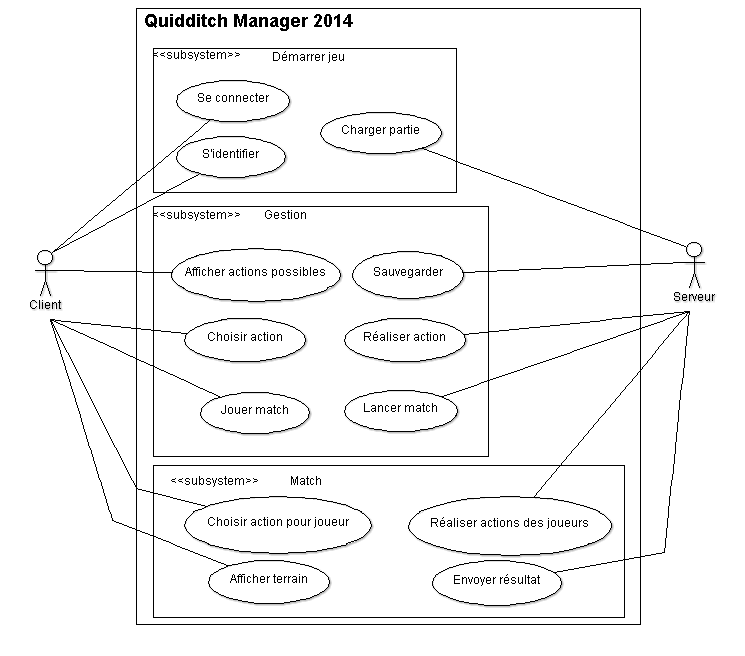
\includegraphics[scale=0.7]{uml/QM2014.png}
    \caption{Cas d'utilisation 1: Quidditch Manager 2014}
  \end{figure}	
    Ce diagramme représente le fonctionnement de base du jeu avec la répartition des "tâches" au niveau serveur et client.
    \subsubsection{Se connecter}
      \begin{itemize}
        \item \textbf{Acteur} : Client.
        \item \textbf{Relations avec d'autres cas d'utilisation}  : Néant.
        \item \textbf{Pré-conditions} : Le serveur doit être connecté.
        \item \textbf{Post-conditions} : Client et serveur sont reliés par le réseau.
        \item \textbf{Cas général} : Le client se connecte au serveur du jeu pour pouvoir jouer. 
        \item \textbf{Cas exceptionnels} : 
        \begin{itemize}
            \item La connexion au serveur échoue. Le programme le signale à l'utilisateur. Ceci termine ce use case.
          \end{itemize}
      \end{itemize}
    \subsubsection{S'identifier}
      \begin{itemize}
        \item \textbf{Acteur} : Client.
        \item \textbf{Relations avec d'autres cas d'utilisation}  : Néant.
        \item \textbf{Pré-conditions} : Le client est connecté au serveur.
        \item \textbf{Post-conditions} : Le client a accès à sa partie.
        \item \textbf{Cas général} : Le client crée une nouvelle \gls{partie}\index{partie} ou en charge une existante pour s’identifier auprès du serveur. Si le client charge une partie existante, le serveur va récupérer le fichier de sauvegarde approprié, sinon, il va en créer un nouveau.
        \item \textbf{Cas exceptionnels} : 
         \begin{itemize}
            \item Le client entre un identifiant ou un mot de passe déjà utilisé. Le programme le signale à l'utilisateur et lui redemande de s'identifier.
          \end{itemize}
      \end{itemize}
    \subsubsection{Charger partie}
      \begin{itemize}
        \item \textbf{Acteur}  : Serveur.
        \item \textbf{Relations avec d'autres cas d'utilisation}  : Néant.
        \item \textbf{Pré-conditions} : La connexion et l'authentification d'un client se sont déroulés sans encombre.
        \item \textbf{Post-conditions} : La partie est chargée.
        \item \textbf{Cas général} : Le serveur va charger les informations de la partie à laquelle va accéder le client.
        \item \textbf{Cas exceptionnels} : 
        \begin{itemize}
            \item Le client ne possède pas encore de partie. Le serveur lui en crée une.
          \end{itemize}
      \end{itemize}
    \subsubsection{Sauvegarder}
      \begin{itemize}
        \item \textbf{Acteur}  : Serveur.
        \item \textbf{Relations avec d'autres cas d'utilisation}  : Néant.
        \item \textbf{Pré-conditions} : Des informations relatives à la partie d'un client ont été modifiées et nécessitent d'être sauvées.
        \item \textbf{Post-conditions} : Les changements sont sauvegardés dans le fichier de sauvegarde dédié au client.
        \item \textbf{Cas général} : Le serveur sauvegarde les informations de la partie. L’état actuel de la partie du client est sauvegardée dans un fichier de sauvegarde.
        \item \textbf{Cas exceptionnels} : Néant.
      \end{itemize}
    \subsubsection{Afficher actions possibles}
      \begin{itemize}
        \item \textbf{Acteur}  : Client.
        \item \textbf{Relations avec d'autres cas d'utilisation}  : Néant.
        \item \textbf{Pré-conditions} : Le client est connecté au serveur.
        \item \textbf{Post-conditions} : Néant.
        \item \textbf{Cas général} : Le client affiche tout ce qu’il est possible de faire d’un point de vue gestion.
        \item \textbf{Cas exceptionnels} : Néant.
      \end{itemize}
    \subsubsection{Choisir action}
      \begin{itemize}
        \item \textbf{Acteur}  : Client.
        \item \textbf{Relations avec d'autres cas d'utilisation}  : Néant.
        \item \textbf{Pré-conditions} : Le client est connecté au serveur.
        \item \textbf{Post-conditions} : La requête a été envoyée au serveur.
        \item \textbf{Cas général} : Le client a choisi une action de gestion à effectuer (amélioration bâtiment, entraînement, publicité, achat, vente, gestion d’équipe). Il doit maintenant attendre que le serveur exécute cette action.
        \item \textbf{Cas exceptionnels} : 
        \begin{itemize}
            \item L'envoi échoue. Le programme le signale à l'utilisateur.
          \end{itemize}
      \end{itemize}
    \subsubsection{Réaliser action}
      \begin{itemize}
        \item \textbf{Acteur}  : Serveur.
        \item \textbf{Relations avec d'autres cas d'utilisation}  : Néant.
        \item \textbf{Pré-conditions} : Client et serveur sont connectés.
        \item \textbf{Post-conditions} : La requête a été traitée par le serveur.
        \item \textbf{Cas général} : Le client a choisi de faire une action de gestion (amélioration bâtiment, entraînement, publicité, achat, vente, gestion d’équipe). Le serveur va se charger de faire les modifications liées à cette action.
        \item \textbf{Cas exceptionnels} :
        \begin{itemize}
            \item La réception échoue. Le programme le signale à l'utilisateur.
          \end{itemize} 
      \end{itemize}
    \subsubsection{Jouer match}
      \begin{itemize}
        \item \textbf{Acteur}  : Client.
        \item \textbf{Relations avec d'autres cas d'utilisation}  : Néant.
        \item \textbf{Pré-conditions} : La date et le moment de la journée correspondent à un match prévu dans le championnat.
        \item \textbf{Post-conditions} : Ce \index{match}match est retiré du \gls{calendrier}\index{calendrier} des matches.
        \item \textbf{Cas général} : On va quitter la partie gestion pour lancer le match. Avant de pouvoir commencer le \index{match}match, le client doit choisir la liste des joueurs qui seront sur le terrain. 
        \item \textbf{Cas exceptionnels} : Néant.
      \end{itemize}
    \subsubsection{Lancer match}
      \begin{itemize}
        \item \textbf{Acteur}  : Serveur.
        \item \textbf{Relations avec d'autres cas d'utilisation}  : Néant.
        \item \textbf{Pré-conditions} : Les deux clients devant s'affronter sont connectés.
        \item \textbf{Post-conditions} : Néant.
        \item \textbf{Cas général} : Le serveur va maintenant gérer le match et l’aspect gestion ne sera plus accessible tant que le match ne sera pas terminé.
        \item \textbf{Cas exceptionnels} : Néant
          %\begin{itemize}
            %\item Un des clients ne s’est pas connecté pour le match, le serveur prendra sa place pour déplacer ses joueurs et affronter le client connecté.
			%\item Aucun client ne s’est connecté pour le match, le match est considéré comme annulé.
          %\end{itemize}    	
      \end{itemize}
    \subsubsection{Choisir action pour joueur}
      \begin{itemize}
        \item \textbf{Acteur}  : Client.
        \item \textbf{Relations avec d'autres cas d'utilisation}  : Néant.
        \item \textbf{Pré-conditions} : Le joueur sélectionné est encore libre de faire une action.
        \item \textbf{Post-conditions} : L'action choisie est réalisée par ce joueur lors du tour.
        \item \textbf{Cas général} : Le client choisit l'action que devra réaliser le joueur lors du tour. Cela peut-être un déplacement et/ou une action particulière comme passer le \index{balle!souafle}souafle ou tirer aux buts. Le client doit faire cela pour chacun de ses joueurs ou indiquer au serveur qu’il a fini de choisir ses actions (s’il souhaite par exemple que des joueurs ne fassent rien).
        \item \textbf{Cas exceptionnels} : 
        \begin{itemize}
         \item Le client ne donne aucune instruction au joueur. Le joueur reste sur place.
        \end{itemize}
      \end{itemize}
    \subsubsection{Réaliser action des joueurs}
      \begin{itemize}
        \item \textbf{Acteur}  : Serveur.
        \item \textbf{Relations avec d'autres cas d'utilisation}  : Néant.
        \item \textbf{Pré-conditions} : Cette action se déroule dans le cadre d'un match.
        \item \textbf{Post-conditions} : La situation sur le terrain a évolué.
        \item \textbf{Cas général} : A chaque tour, le serveur attend de recevoir les actions que les clients ont choisies pour chacun de leurs joueurs. Une fois l’ensemble de ces actions reçues, le serveur les exécute puis envoie la nouvelle situation aux clients. Les clients affichent alors le terrain et redemandent les actions à exécuter aux utilisateurs.
        \item \textbf{Cas exceptionnels} : 
          \begin{itemize}
            \item Si un des clients ne s’est pas connecté pour le match, le serveur n’attendra pas d’actions de la part de ce client. Ses joueurs suivront une stratégie automatique minimaliste prise en charge par le serveur.
          \end{itemize}  
      \end{itemize}
    \subsubsection{Afficher terrain}
      \begin{itemize}
        \item \textbf{Acteur}  : Client.
        \item \textbf{Relations avec d'autres cas d'utilisation}  : Néant.
        \item \textbf{Pré-conditions} : Le client est connecté au serveur et un match a lieu.
        \item \textbf{Post-conditions} : Néant.
        \item \textbf{Cas général} : Le client reçoit les informations relatives au \index{terrain}terrain de la part du serveur et l’affiche pour permettre au client de facilement visualiser la situation actuelle du jeu.
        \item \textbf{Cas exceptionnels} : Néant. 
      \end{itemize}
    \subsubsection{Envoyer résultat}
      \begin{itemize}
        \item \textbf{Acteur}  : Serveur.
        \item \textbf{Relations avec d'autres cas d'utilisation}  : Néant.
        \item \textbf{Pré-conditions} : Le match est terminé.
        \item \textbf{Post-conditions} : Le client dispose des informations à afficher après un match.
        \item \textbf{Cas général} : Le match est terminé. Le serveur va calculer combien le Manager a gagné (en fonction des bâtiments \gls{fanshop}\index{bâtiment!FanShop} (match à domicile) ou \gls{buvette}\index{bâtiment!Buvette} (match en extérieur)). En fonction de la situation de fin de match, victoire ou défaite, le serveur va également déterminer combien d’argent et de popularité le Manager a gagné ou perdu. Toutes ses informations sont envoyées au client.
        \item \textbf{Cas exceptionnels} : Néant.
      \end{itemize}

\section{Exigences non fonctionnelles}
  \subsection{Le réseau}
  Au niveau du réseau, le problème de la synchronisation n'est pas préoccupant, 
  car le client ne sera qu'une interface d'affichage et d'interaction. 
  Pour ce qui est de la quantité d'informations échangées, 
  elle ne devrait pas être très importante pour autant, 
  les éléments à afficher et leur diversité étant relativement réduits.
  
  Il faudra veiller à ce que l'interaction avec l'utilisateur soit transparente 
  au niveau du serveur, à travers une classe de message générique, 
  que le programme client instanciera de la même manière, 
  qu'il tourne à travers une interface graphique ou à travers le terminal.
  \subsection{Performance}
  Pour ce qui est de la performance, la localisation de tous les calculs sur la machine serveur 
  implique une centralisation de la puissance de calcul. 
  D'un autre côté, le client ne nécessitera que très peu de puissance de son côté pour pouvoir jouer.
  \subsection{Sécurité}
  La sécurité d'une partie sera assurée par l'identification : 
  seul un utilisateur identifié peut charger une partie, et la sienne uniquement.
  \subsection{Environnement d'exécution}
  L'environement d'exécution étant fixé (les machines des salles informatiques du NO), 
  le code se limitera à l'utilisation des librairies C++ standards. 
  Le système d'exploitation visé est GNU/Linux.
  \subsection{Choix d'une librairie graphique}
  Qt est un framework d'interface graphique orienté objet et développé en C++ par la PME norvégienne Trolltech.
La première version gratuite fut mise à disposition du public en mai 1995\cite{Blanchette2006}. \\
Il offre des composants d'interface graphique (widgets), d'accès aux données, de communication réseau, de gestion des threads. \\
Il permet la portabilité des applications qui n'utilisent que ses composants par simple recompilation du code source.
Les environnements supportés sont les Unix (dont Linux) qui utilisent le système graphique X Window System, Windows et Mac OS X,
mais aussi Android, iOS et QNX (BlackBerry). \\
Il peut s'intégrer dans des développements réalisés dans la plupart des langages de programmation modernes, d'Ada à Python. \\
Ses librairies sont accompagnées de plusieurs outils de développement, parmi lesquels :
\begin{itemize}
\item Un IDE;
\item Un concepteur d'interface graphique;
\item Des plugins pour Eclipse et Visual Studio.
\end{itemize}

Qt est notamment connu pour être la bibliothèque sur laquelle repose l'environnement graphique KDE, l'un des environnements de bureau les plus utilisés dans le monde Linux;
des logiciels commerciaux comme Adobe Photoshop Album, Autodesk Maya et Mathematica, et
des logiciels gratuits omniprésents comme Skype, VLC media player et VirtualBox, l'utilisent également. \\
La popularité de Qt (des milliers de clients et des dizaines de milliers de programmeurs) est un point important dans le choix de la bibliothèque graphique.
Elle permet en effet d'assurer :
\begin{itemize}
\item Sa pérennité et son adaptation aux évolutions technologiques;
\item Sa fiabilité et la qualité de son support;
\item Une communauté d'utilisateurs actifs sur de nombreux forums d'entraide;
\item Une documentation abondante et de qualité.
\end{itemize}

\section{Design et fonctionnement du système}
  % Cette partie sera décrite à l’aide des différents diagrammes UML
  % vus au cours théorique et aux exercices.
  \subsection{Le jeu sur terminal}
Nous allons ici décrire comment se déroule une partie sur terminal. Nous pouvons tout d'abord distinguer 2 parties différentes, la gestion et le match.
\textbf{Gestion} : La partie gestion du jeu permet donc au Manager, le client, de gérer une équipe ainsi qu'un domaine. Ce domaine se compose de plusieurs bâtiments, ayant chacun leur particularité et avantage. Le Manager peut donc se balader au travers des différents menus qui lui permettent d'accéder aux informations de ses joueurs (leurs capacités, etc) et de ses bâtiments et d'effectuer des actions de gestion telles qu'entraîner ou soigner un joueur, participer à une enchère ou améliorer un bâtiment. \\
\textbf{Match} : A tout moment, s'il possède au moins 7 joueurs disponibles, le Manager peut envoyer une demande de match amical à un autre client connecté. Si la réponse de ce dernier est positive, le match débutera. Ce match de Quidditch se déroule au tour par tour. Chacun de leur côté, les adversaires choisissent les mouvements qu'ils veulent que leurs joueurs fassent, sans savoir ce qu'a préparé l'autre manager. Et ainsi de suite jusqu'à une situation de fin de partie. \\

  \subsection{Implémentation}
  
  Dans cette partie sera expliquée l'implémentation générale du jeu; de quelles façons les fonctionnalités ont été mises en place, les choix faits, etc. Des diagrammes de classes viendront détailler ces explications.
    \begin{landscape} %mode paysage
    \begin{figure}[H]
      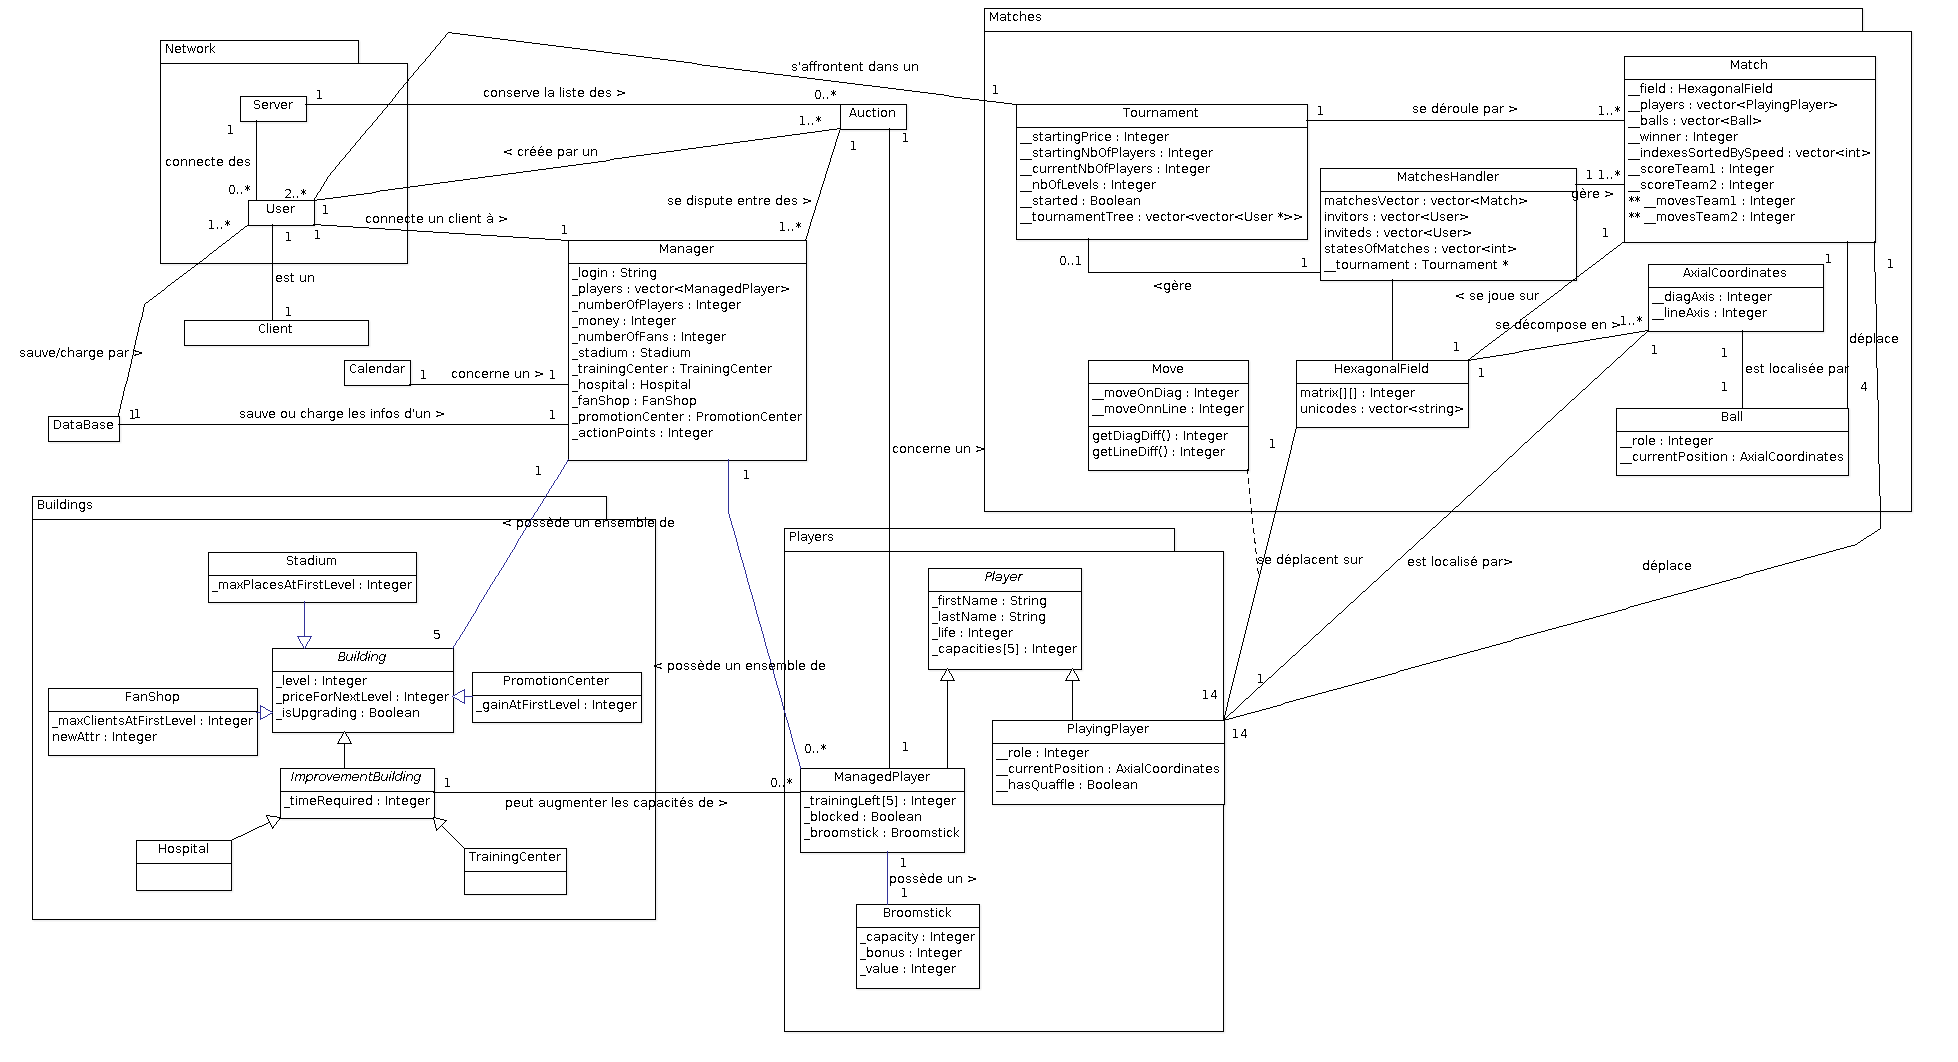
\includegraphics[scale=0.35]{uml/class/Global.png}%<---angle here
      \caption{Diagramme de classes global}
    \end{figure}
    \end{landscape}

      \subsubsection{Gestion générale}
          \begin{figure}[H]
          \center
          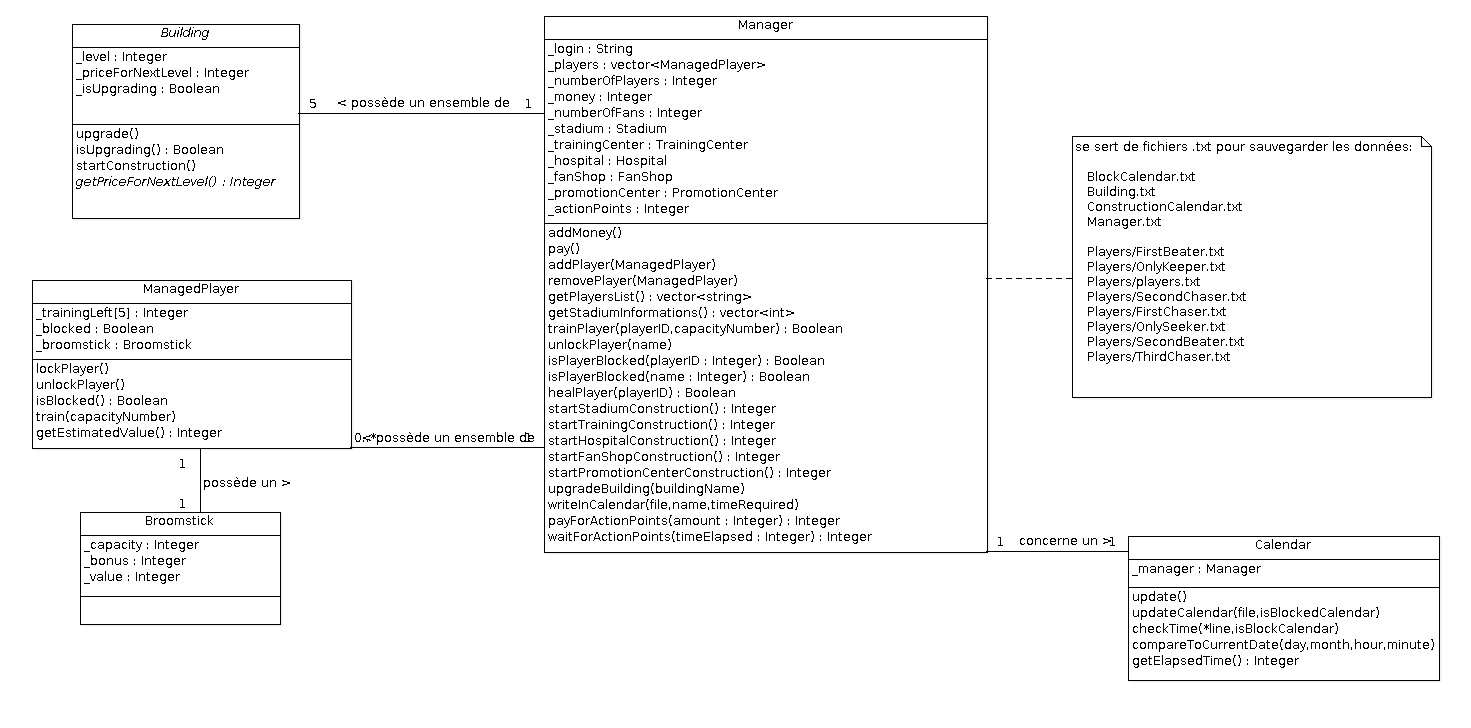
\includegraphics[scale=0.35]{uml/class/Management.png}
         \caption{Diagramme des classes impliquées dans la gestion générale}
         \end{figure}

        Un manager est le \"personnage virtuel\" qu'incarne un client. Il est le propriétaire d'un domaine et d'une équipe de quidditch. Au départ du jeu, il possède quelques bâtiments sur son domaine, et sept joueurs de qualité moyenne, si pas médiocre. Pour améliorer ses bâtiments, ou les capacités de ses joueurs, le manager doit dépenser des points d'action, de l'argent, et attendre. L'attente en temps réel est gérée par la classe Calendrier.


      \subsubsection{Bâtiments}
          \begin{figure}[H]
          \center
          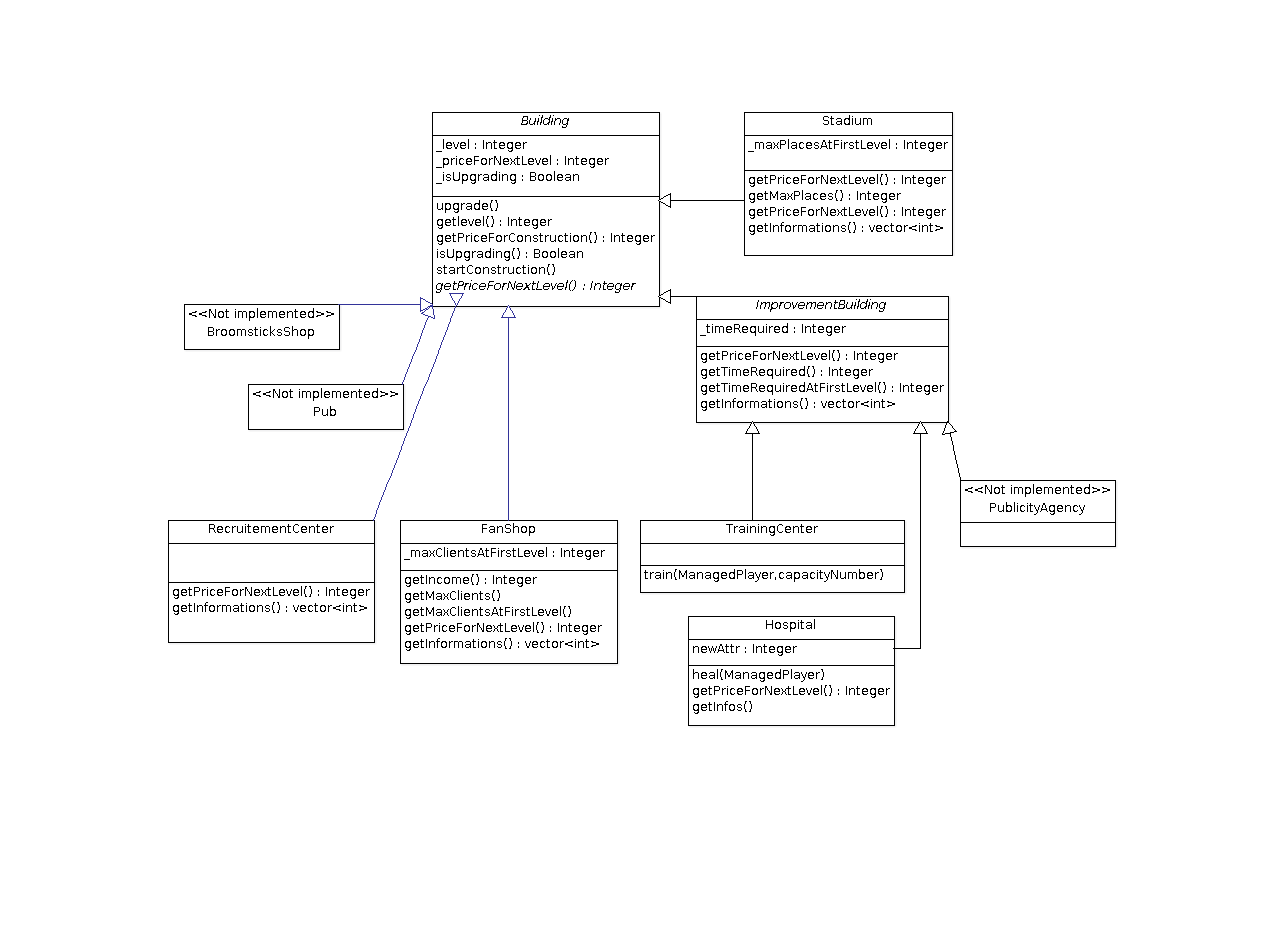
\includegraphics[scale=0.4]{uml/class/Buildings.png}
         \caption{Diagramme des classes pour les bâtiments}
         \end{figure}

        Le domaine du manager contient 5 emplacements pour chacun des bâtiments qu’il peut posséder. Au début du jeu, 4 des 5 bâtiments sont déjà au niveau, seul le fan shop n’est pas encore construit.\\

        Les 5 bâtiments sont :
        \begin{itemize}
        \item Le stade : Il s’agit du lieu dans lequel se joueront les matches. La capacité en spectateurs ainsi que le nombre de fans du manager déterminent l’argent gagné lorsqu’un match a lieu dans le stade. La capacité augmente avec les niveaux.
        \item Le centre d’entraînement : C’est ici que viennent s’entraîner les joueurs pour améliorer leurs capacités. La durée d’une session d’entraînement, et de son blocage, diminue quand le niveau du bâtiment augmente.
        \item L’hôpital : C’est ici que le manager envoie ses joueurs blessés (suite à un match) pour qu’ils soient soignés. La durée des soins, et du blocage, diminue quand le niveau du bâtiment augmente.
        \item Le fan shop : Il s’agit d’un magasin qui vend des produits aux couleurs de l’équipe du manager. A chaque match à domicile, un certain nombre de fans pourra se rendre dans le magasin et y faire des achats. La recette dépend donc de ce nombre, qui est déterminé par le niveau du bâtiment.
        \item Le centre de promotion : C’est ici que le manager peut venir récupérer des points d’action gratuitement. Au lieu de payer, il attend un certain temps pour recevoir des points actions. Le niveau du bâtiment détermine combien de points d’action il gagne en attendant x minutes (ce nombre de minutes étant lui-même défini dans le code, il peut facilement être changé).
        \end{itemize}

      \subsubsection{Joueurs}
          \begin{figure}[H]
          \center
          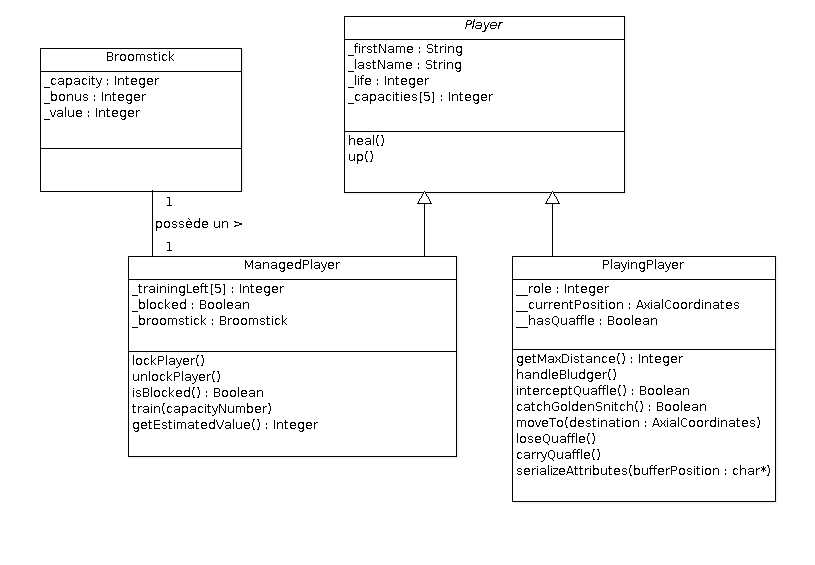
\includegraphics[scale=0.4]{uml/class/Players.png}
         \caption{Diagramme des classes pour les joueurs}
         \end{figure}

        Du point de vue de l'implémentation, les joueurs sont différenciés s'ils sont en phase de gestion ou en train de jouer un match, d'où les deux classes ManagedPlayer, pour la gestion, et PlayingPlayer, pour les matches. La seule différence entre les deux est que le bonus lié au balai (actuellement toujours à 0) est absorbé dans les capacités du joueur telles qu'elles sont vues pendant un match.\\
\\
        Un joueur se distingue des autres par son nom, choisi au hasard à la création du joueur. Les différents postes que peuvent occuper les joueurs, à savoir attrapeur, gardien, poursuiveur et batteur, ne sont pas prédéterminés. Le manager peut choisir à quel poste faire jouer ses joueurs avant chaque match. Néanmoins, dans un souci d'équité, lors de la création de l'équipe de base (nouvelle partie), les joueurs par défaut attribués au client présentent des capacités axées sur un poste particulier. \\

        Les capacités, ou caractéristiques des joueurs, sont les suivantes :
        \begin{itemize}
        \item La vitesse, qui détermine la longueur maximale des déplacements lors d'un match
        \item La force, qui détermine l'aptitude des batteurs à frapper un cognard
        \item La précision, qui intervient dans les passes, les tirs, etc.
        \item Les réflexes, pour attraper le vif d'or, intercepter le souafle, etc.
        \item La résistance, qui détermine la "vie" du joueur, ou combien de coups de cognard il peut recevoir avant d'être incapable de poursuivre le match.
        \end{itemize}

        Les joueurs possèdent également un balai (c'est en effet plus pratique pour voler) qui, s'il est de qualité, booste un de ces 5 attributs (fonctionnalité non implémentée mais envisagée).\\

        Pour pouvoir améliorer les capacités de ses joueurs, un manager peut les envoyer s'entraîner. Pour augmenter une capacité et passer au niveau suivant, le joueur devra réaliser un certain nombre de sessions d'entraînement, ce nombre étant déterminé par le niveau actuel de la capacité concernée.\\

        Enfin, lorsque la vie du joueur n'est pas optimale, le manager peut l'envoyer à l'hôpital se faire soigner.


      \subsubsection{Sauvegarde et chargement}
          \begin{figure}[H]
          \center
          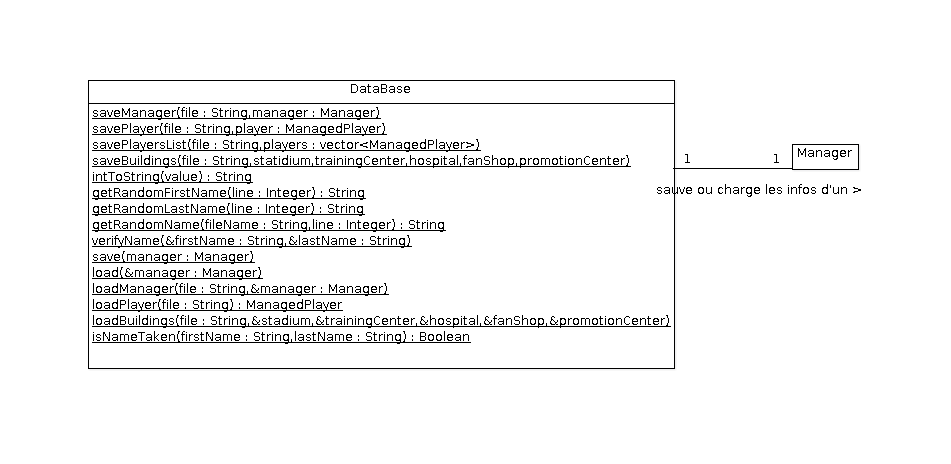
\includegraphics[scale=0.4]{uml/class/DataBase.png}
         \caption{Diagramme de classes pour les sauvegardes/chargements}
         \end{figure}

        La structure des fichiers de sauvegarde se présente comme suit : \\

        A chaque client est associé un dossier de sauvegarde portant le nom de son compte ; son login.
        Dans ce dossier se trouvent des fichiers .txt : un se nommant selon son login (donc un format login.txt), buildings.txt, blockCalendar.txt et constructionCalendar.txt\\

        Le fichier login.txt contient les informations relatives aux attributs de l’objet Manager, c’est-à-dire le nombre de joueurs possédés, l’argent, le nombre de fans et le nombre de points d’action que le client a. Le format du fichier est donc :\\
       
       \begin{itemize}  
        \item Nombre de joueurs
        \item Argent
        \item Nombre de fans
        \item Nombre de points d’action
        \end{itemize} 

         
         Le fichier buildings.txt contient les informations relatives à chaque bâtiment du client ; le stade, le centre d’entraînement, l’hôpital, le fan shop et le centre de promotion. Il y a 4 informations pour chaque bâtiment : son niveau actuel, le prix pour la construction (passage du niveau 0 au niveau 1), la valeur au niveau 1 de l’attribut particulier à chaque bâtiment et un indicateur de projet (0 si le bâtiment est libre, 1 si on a lancé une construction ou une amélioration et qu’elle n’est pas encore terminée). Le format du fichier est donc :\\

          \begin{itemize}
            \item Niveau du stade
            \item Prix de construction du stade
            \item Nombre de places dans le stade au niveau 1
            \item Indicateur de projet
            \item Niveau du centre d’entraînement
            \item Prix de construction du centre d’entraînement
            \item Durée du blocage en tours au niveau 1
            \item Indicateur de projet
            \item Niveau de l’hôpital
            \item Prix de construction de l’hôpital
            \item Durée du blocage en tours au niveau 1
            \item Indicateur de projet
            \item Niveau du fan shop
            \item Prix de construction du fan shop
            \item Nombre de clients max dans le fan shop au niveau 1
            \item Indicateur de projet
            \item Niveau du centre de promotion
            \item Prix de construction du centre de promotion
            \item Nombre de points d’action gagnés par tranche de temps au niveau 1
            \item Indicateur de projet
        \end{itemize}

        Le fichier blockCalendar.txt contient les informations concernant les blocages des joueurs quand ceux-ci sont à l’hôpital ou à l’entraînement. Chaque ligne représente un blocage et a donc le nom du joueur concerné, la date de début du blocage ainsi que la durée en minutes de ce blocage. Le format d’une ligne du fichier est donc :\\

          \begin{itemize}
            \item Prénom Nom\#Date de début (au format jour:mois:heure:minute)\#Durée du blocage\#
          \end{itemize} 

        Le fichier constructionCalendar.txt contient les informations concernant les projets de construction ou d’amélioration des bâtiments. Chaque ligne correspond à un projet et a donc le nom du bâtiment concerné, la date de début de construction ou d’amélioration et la durée en minutes du projet. Le format d’une ligne du fichier est donc :\\

          \begin{itemize}
            \item Nom du bâtiment\#Date de début (au format jour:mois:heure:minute)\#Durée du projet\#
          \end{itemize} 

        En plus de ces 4 fichiers, le dossier de sauvegarde du client contient un sous-dossier nommé Players. Ce sous-dossier contient un fichier players.txt qui est une liste de tous les autres fichiers contenus dans ce sous-dossier. Ces autres fichiers « PrénomNom.txt » correspondent chacun à un joueur de l’équipe du client et possèdent toutes les informations relatives à ce joueur. Le fichier players.txt permet donc de savoir quels fichiers il faut lire quand on va charger une partie.\\

        Un fichier de joueur, PrénomNom.txt contient donc les informations du joueur, c’est-à-dire ses capacités, l’avancement de ses entraînements, etc. Le format est le suivant :\\

          \begin{itemize}
            \item Prénom
            \item Nom
            \item Vitesse
            \item Force 
            \item Précision
            \item Réflexe 
            \item Résistance
            \item Vie
            \item Nombre de sessions d’entraînement à faire avant d’améliorer la vitesse
            \item Nombre de sessions d’entraînement à faire avant d’améliorer la force
            \item Nombre de sessions d’entraînement à faire avant d’améliorer la précision
            \item Nombre de sessions d’entraînement à faire avant d’améliorer le réflexe
            \item Nombre de sessions d’entraînement à faire avant d’améliorer la résistance
            \item 1 si le joueur est bloqué ou 0 sinon 
            \item Indice de la capacité pour laquelle le balai offre un bonus
            \item La valeur du bonus offert par le balai
          \end{itemize}


      \subsubsection{Enchères}
          \begin{figure}[H]
          \center
          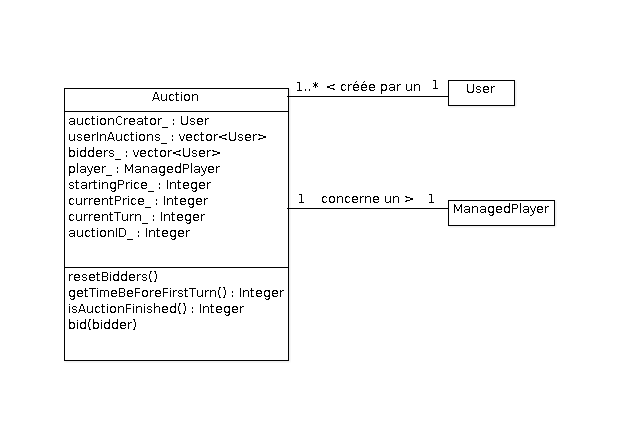
\includegraphics[scale=0.4]{uml/class/Auction.png}
         \caption{Diagramme de classes pour les enchères}
         \end{figure}

        Les enchères se déroulent au tour par tour. A chaque tour, les managers désireux de poursuivre la vente doivent enchérir. S'ils ne le font pas dans le temps imparti, ou qu'ils souhaitent quitter l'enchère, ils devront attendre la fin du tour avant d'avoir à nouveau accès aux menus de jeu. Le dernier tour est atteint quand il n'y a plus qu'un seul manager qui enchérit, il gagne alors la vente.
        Pour gérer le temps imparti par tour, la solution adoptée est l'utilisation de threads. Le thread principal lance à chaque début de tour un thread sur une méthode qui enregistre le choix du manager (enchérir ou non). Après avoir lancé ce thread secondaire, le thread principal s'endort pour une durée déterminée. A son réveil, il invite cordialement l'autre thread à s'arrêter. Le tour est fini et les managers ne peuvent plus enchérir. On répète donc cela jusqu'à ce qu'il n'y ait plus qu'un seul manager à avoir enchéri.

      \subsubsection{Matches}
          \begin{figure}[H]
          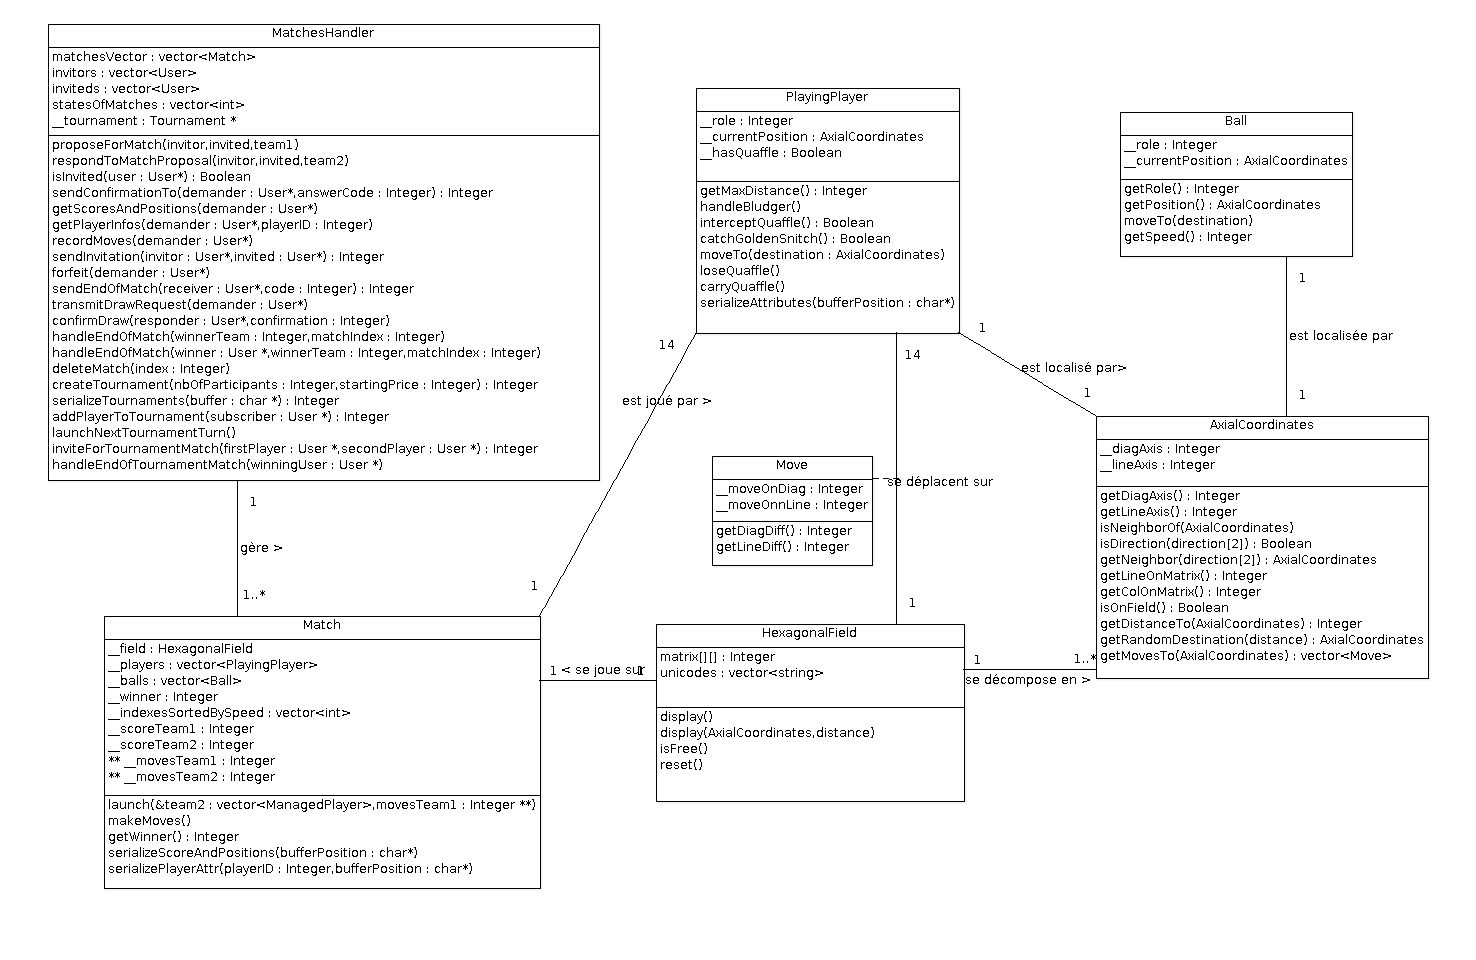
\includegraphics[scale=0.35]{uml/class/Match.png}
         \caption{Diagramme de classes pour les matches}
         \end{figure}

            Le match relie deux clients différents dans un affrontement sur un \gls{terrain}\index{terrain} où se déplacent à la fois des joueurs et des \index{balle}balles, les joueurs pouvant faire se déplacer les balles. Le terrain est représenté par un hexagone allongé et respecte le format \"case hexagonale\", c'est-à-dire qu'il y a 6 cases de destination adjacentes à une case donnée (si elle n'est pas sur les bords). Un client peut participer à deux \"types\" de match, soit un match amical, en invitant un autre joueur ou en étant invité, soit un match de tournoi, qui offre des récompenses plus importantes. Au début de chaque match, le client choisit quels joueurs seront sur le terrain, et à quel poste ils joueront. Le déroulement des matches consiste en du tour par tour.

      \subsubsection{Tournois}
          \begin{figure}[H]
          \center
          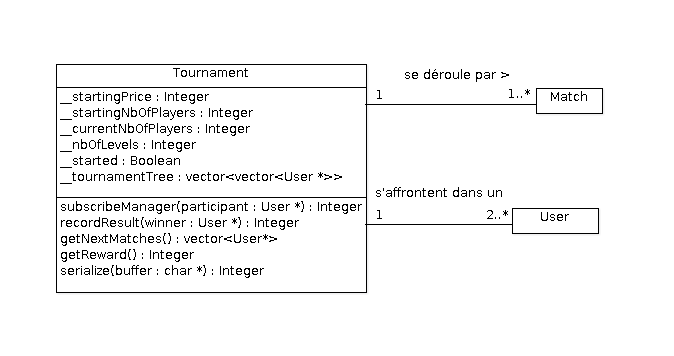
\includegraphics[scale=0.4]{uml/class/Tournament.png}
         \caption{Diagramme de classes pour les tournois}
         \end{figure}

         A compléter.
        
      \subsubsection{Réseau}
          \begin{figure}[H]
          \center
          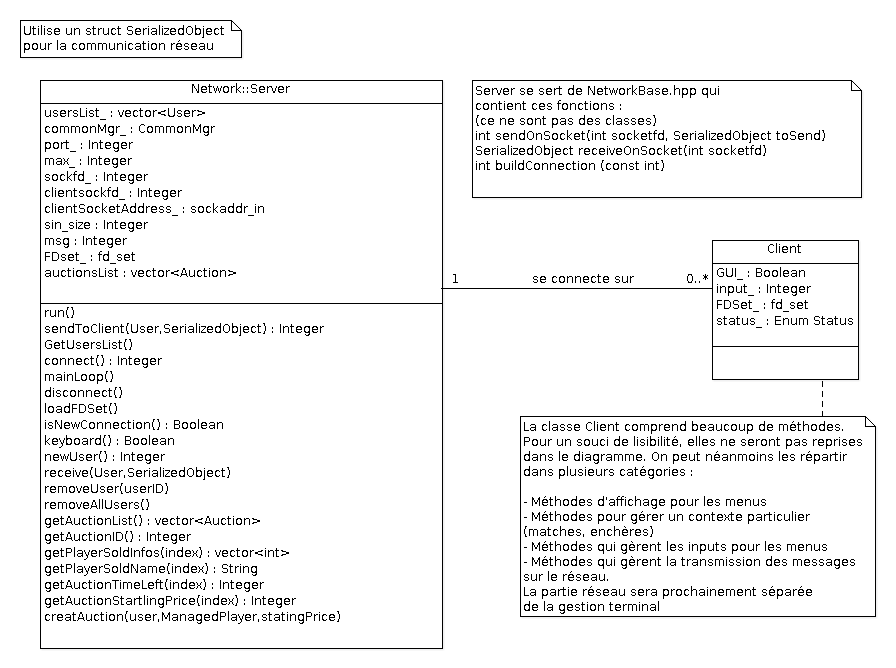
\includegraphics[scale=0.4]{uml/class/Server.png}
         \caption{Diagramme de classes pour le serveur}
         \end{figure}

        
          \begin{figure}[H]
          \center
          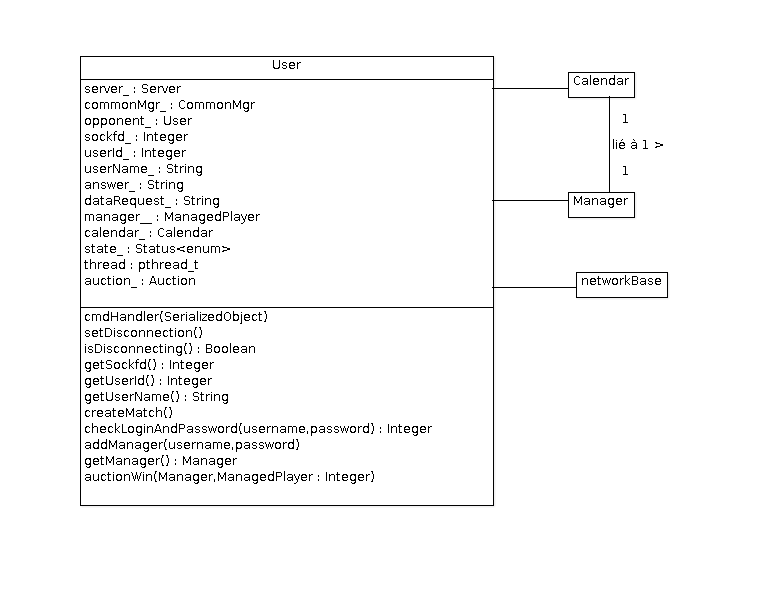
\includegraphics[scale=0.35]{uml/class/User.png}
         \caption{Diagramme de classes pour les utilisateurs sur le réseau}
         \end{figure}

          La relation avec le client est gérée par une classe principale, qui va assurer la communication
          à travers une classe de messages (un \emph{struct} puisque la base réseau consiste en des appels systèmes C).
          C'est cette classe principale qui va gérer les alternances entre le côté gestion et le côté match. Le match nécessite une connexion entre deux clients, elle est donc très différente de la gestion
          à ce niveau-là aussi.

      \subsubsection{Interface graphique}
      \begin{figure}[H]
          \center
          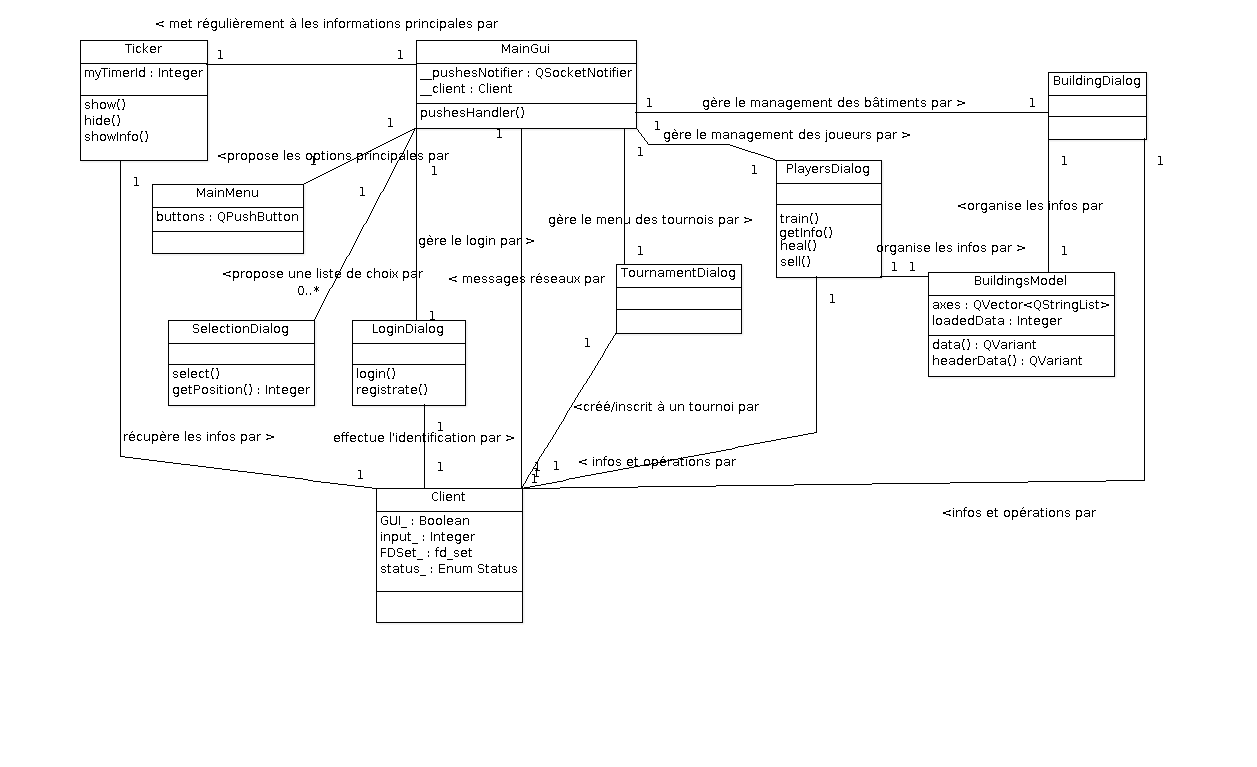
\includegraphics[scale=0.4]{uml/class/GUIClasses.png}
         \caption{Diagramme des classes impliquées dans la GUI}
         \end{figure}
         
         Une fenêtre principale fait appel à différentes sous-fenêtres pour des interactions particulières.
         Si une fenêtre a besoin de communiquer avec le serveur, elle le fera à travers un pointeur de la classe Client,
         la fenêtre principale instanciant une classe client à sa construction.\\
         
    Pour une description plus élaborée de la partie graphique, le lecteur se reportera utilement au § \ref{diag-client-graphique}.
    
\subsection{Le réseau}
  L'interface réseau doit permettre une communication bidirectionnelle :
\begin{itemize}
  \item des clients chargés de communiquer chacun avec un User : affichage d'informations et enregistrement de commandes;
  \item un serveur chargé de partager de l'information entre les clients en la centralisant et en la conservant sur disque.
\end{itemize}
La logique applicative peut être répartie entre ces deux entités, comme elle peut être concentrée sur le serveur (le client se comporte alors comme un browser sans scripts) ou sur le client (le serveur peut se limiter aux fonctions de gestionnaire de fichiers ou de bases de données et de données temporaires en mémoire centralisée).\\
Entre les deux, l'interface réseau, comme tout middleware, ne doit pas connaître les formats internes des messages échangés entre clients et serveur. Le respect de ce principe doit permettre d'assurer à la fois l'indépendance entre le fonctionnel et le technique, et une séparation du code réalisé pour couvrir ces deux aspects du projet.\\
En général, le modèle client-serveur \cite{Bulfone} est serveur-centrique :
\begin{itemize}
  \item les clients ne communiquent qu'avec le serveur, pas entre eux; le partage d'informations entre les clients
  se fait donc via le serveur, selon un modèle de tableau d'affichage (tableau noir), partagé par les/certains clients;
  \item la communication et les dialogues qui s'en suivent se font à l'initiative des clients.
\end{itemize}
Ce deuxième principe ne permet cependant pas de répondre à tous les besoins exprimés pour ce projet :
les clients doivent pouvoir être invités dans des dialogues; ils doivent donc être en mesure,
lorsqu'ils ne sont pas occupés par une activité, de recevoir des messages non sollicités;
nous avons donc dû revoir notre design initial en conséquence, tel qu'il apparaîtra ci-après.\\

\subsubsection{Echange de messages serveur-client}
Les messages échangés entre la partie serveur et la partie client du projet sont transmis selon un principe de sérialisation et désérialisation qui permet de faire transiter sur le réseau des messages totalement différents qu'on identifie par un en-tête. Cet en-tête permet au code qui reçoit ce message de savoir comment le traiter.

 On constate donc la présence de deux structures de séquencement fort similaires, en forme de rateau :
 \begin{itemize}
   \item un input;
   \item le choix d'une séquence d'instruction (une méthode) en fonction de cet input;
   \item un output.
 \end{itemize}
 \begin{algorithm}
  \caption{Traitement séquentiel partagé par le serveur et le client}
  \begin{algorithmic}
  \REQUIRE socket(s) ouvert(s)
  \STATE écoute sur les sockets ouverts et sur le flux d'entrée
  \IF{input sur flux d'entrée}
  \STATE traitement : a l'initiative
  \ELSE[message sur le socket]
  \STATE traitement : sollicité
  \ENDIF
\end{algorithmic}
\label{pseudo-code-select}
\end{algorithm}

\subsubsection{Synopsis du serveur}
\begin{itemize}
  \item Au démarrage, le serveur crée une instance de la classe \emph{MatchesHandler}, destinée à gérer l'interconnexion
   de clients au travers du serveur dans le cas des matchs;
  \item Le serveur se met en attente (fonction select()) d'une activité sur son clavier
  (pour commander l'arrêt du serveur par exemple ou obtenir la liste des utilisateurs connectés...), sur
  son socket destiné à recevoir les nouvelles connexions et sur les sockets des clients déjà connectés (voir diagrammes);
  \item Lors d'une nouvelle connexion, le serveur crée une instance de la classe User; il y a donc un objet User par client;
  \item Tout nouveau message reçu par le serveur est confié à la méthode \emph{commandHandler} de l'objet de type User, qui assure le dispatching
  vers le module fonctionnel concerné, en se basant et mettant à jour la variable d'état state;
  \item Cela assure un contrôle global des activités du client (et de l'arrêt de celles-ci).
  Remarquons que cela pourrait permettre d'entreprendre plusieurs activités en parallèle.
\end{itemize}
    \begin{figure}[H]
    \center
    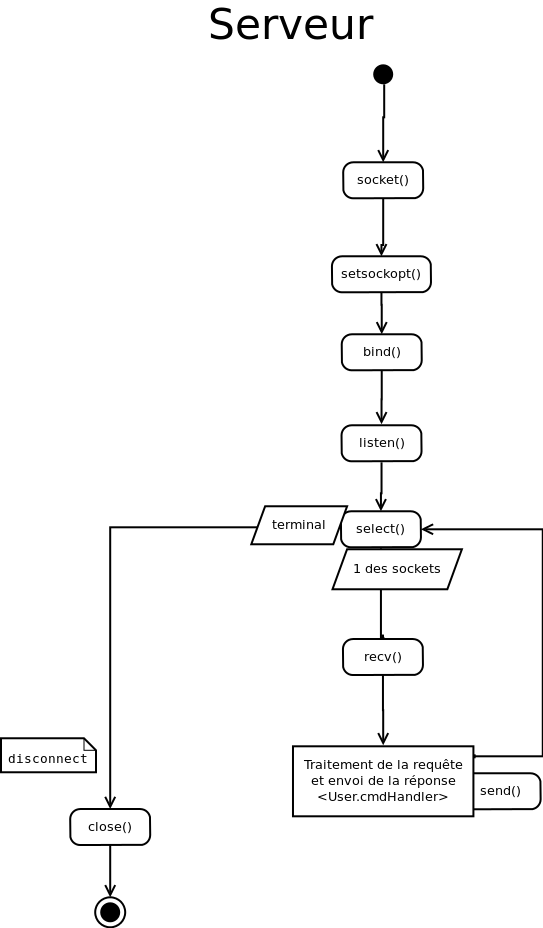
\includegraphics[scale=0.4]{uml/Serveur.png}
    \caption{Diagramme d'activité : cycle de vie du serveur} \label{diag-serveur}
    \end{figure}
Aucune des méthodes du serveur n'étant bloquante pendant plus d'une fraction de seconde (peu d'I/O) et compte tenu des délais très courts pour la mise en œuvre, nous avons opté à ce stade pour une solution mono-thread;
travailler avec un seul thread supprime la nécessité de devoir gérer l'accès concurrent aux données (en mémoire ou sur disque) et la communication entre threads (arrêt du serveur par exemple) :
une solution multi-threads rendrait la gestion de ressources communes par les fonctions applicatives plus complexe (sérialisation de sections critiques), 
tout en étant beaucoup plus gourmande en ressources CPU et présentant des risques de deadlocks (tests plus délicats à réaliser!). 
Pour la gestion des time-out (dans le cas d'une enchère uniquement jusqu'à présent), 
cela est actuellement géré au niveau client par un thread de cadencement (qui ne tourne que le temps d'un tour),
mais cela pourra évoluer vers une utilisation du paramètre temporel de l'appel système \emph{select}.

Si les messages sont de longueur fixe prévisible, un buffer de taille fixe peut être utilisé de part et d'autre.
Sinon (par exemple pour une liste), deux solutions sont possibles :
\begin{itemize}
  \item Envoyer une série de messages de taille fixe;
  \item Utiliser de part et d'autre des zones de mémoire allouées dynamiquement et envoyer tout en un seul message, après un premier message indiquant au client la taille du buffer.
\end{itemize}
Jusqu'à présent nous allouons un buffer de taille fixe.

  \subsubsection{Synopsis du client}
Comme le serveur, le client utilise la fonction select() afin de pouvoir capter indifféremment des messages d'origine différente,
 en l’occurrence en provenance du clavier ou du socket de communication, ceci pour pouvoir recevoir des messages non sollicités dans une solution mono-thread.
      \begin{figure}[H]
    \center
    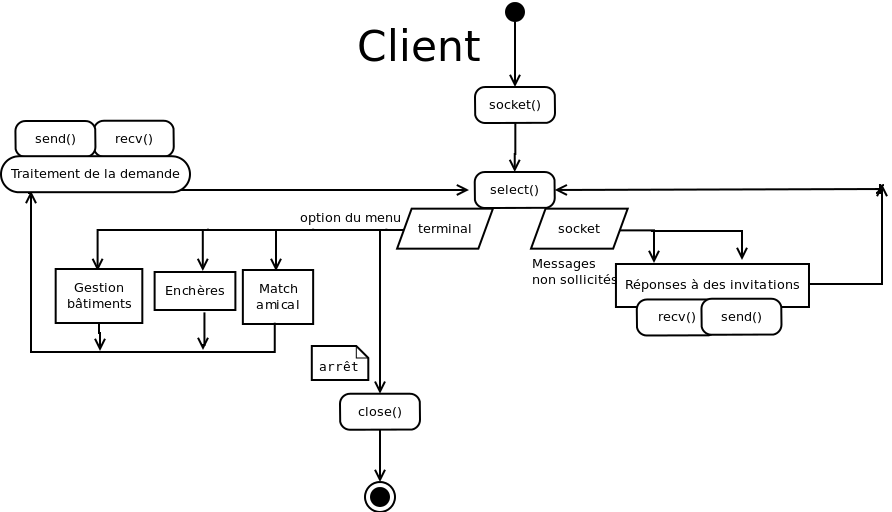
\includegraphics[scale=0.4]{uml/Client.png}
    \caption{Diagramme d'activité : cycle de vie du client} \label{diag-client}
    \end{figure}
 La disponibilité aux messages non sollicités ne peut exister que lorsque le client
 n'est pas dans un contexte verrouillé, c'est-à-dire dans les menus principaux ou au début du tour d'un match.
 
 Lorsque le manager choisit une activité, le client entre dans un dialogue avec à la fois le serveur et le manager,
 sans qu'il puisse être interrompu par un message non sollicité; d'ailleurs, le serveur ne va pas lui en envoyer,
 puisqu'il connaît l'état dans lequel se trouve le client.
 
 Le serveur travaillant en mode répétitif (pas de parallélisme), la variable d'état suffit donc à contrôler l'accès
 aux sections critiques que sont les différentes activités.
 
 De même, lorsque le client reçoit un message non sollicité, il entre dans un dialogue avec à la fois le serveur et le manager,
 sans qu'il puisse être interrompu par un autre message non sollicité ou par une autre demande du manager au clavier.
 
  \subsubsection{Exemples}
    \begin{figure}[H]
    \center
    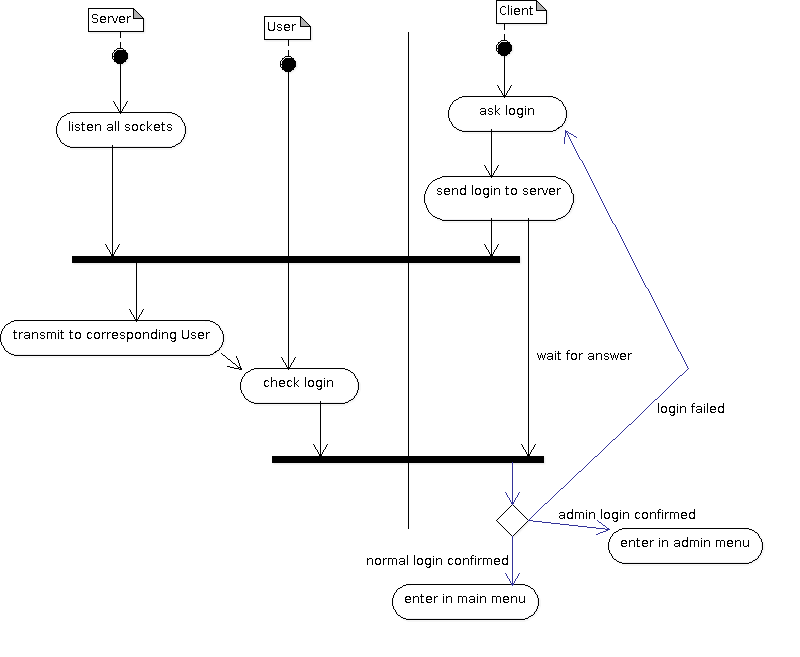
\includegraphics[scale=0.4]{uml/Activity_Login.png}
    \caption{Exemple d'interaction par diagramme d'activité : identification} \label{diag-login}
    \end{figure}
    Cas où le client prend l'initiative de la communication : le code client récupère les identifiants et les envoie au serveur.
    Celui-ci transmet la requête à l'instance User correspondante qui va traiter la demande et communiquer la confirmation au client.
    En fonction de cette confirmation, le code client fera évoluer son contexte et affichera le menu adapté.
    \begin{figure}[H]
    \center
    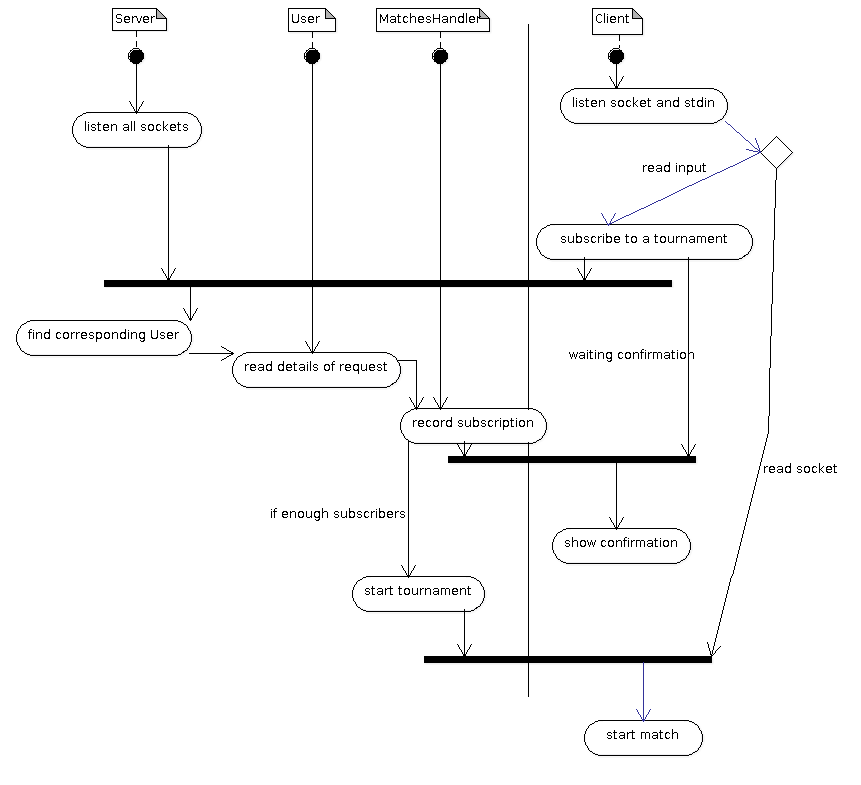
\includegraphics[scale=0.4]{uml/Activity_Tournamentmatch.png}
    \caption{Exemple d'interaction par diagramme d'activité : démarrage d'un tournoi} \label{diag-tournament}
    \end{figure}
    L'inscription et le démarrage d'un tournoi impliquent les deux modes du client : l'initiative et la sollicitation.
    L'inscription se fait par l'input reçu sur le flux d'entrée, par lequel l'utilisateur donne ses instructions.
    L'enregistrement de cette inscription est similaire au processus d'identification, à la différence
    qu'une instance commune à tous les \emph{Users} se charge du traitement et de la réponse.
    
    Quand le nombre d'inscrits requis est atteint, le serveur va inviter les clients à jouer leur match.
    Dans ce cas, le serveur prend l'initiative d'une communication vers le client et c'est le client
    qui va devoir confirmer en envoyer l'équipe de joueurs choisie.
    
    


\subsubsection{Diagramme de séquence}
  Voici un diagramme de séquence qui illustre les relations entre différents objets du code serveur
  et du code client, dans le cas d'un match amical.
    \begin{figure}[H]
    \center
    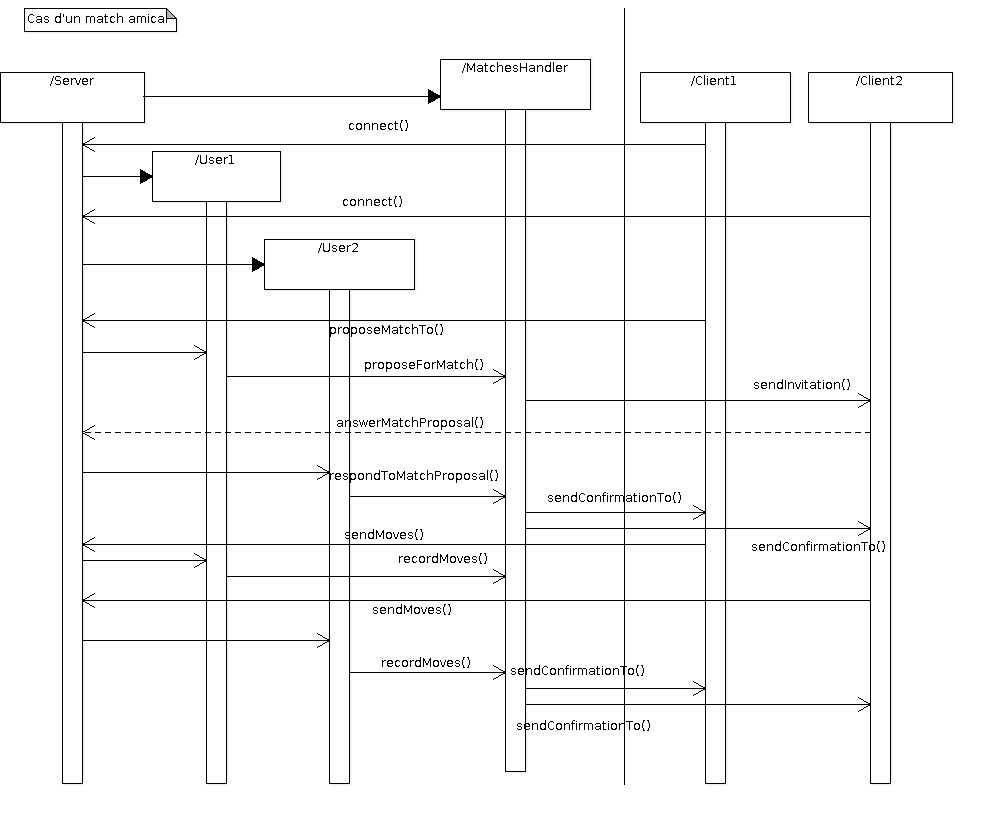
\includegraphics[scale=0.4]{uml/Sequence_matchStarting.png}
    \caption{Diagramme de séquence : démarrage d'un match amical}
    \end{figure}
  À la connexion d'un client, le serveur instancie un User, classe chargé d'interpréter
  les messages reçus sur le socket de communication correspondant.
  Si cette requête concerne la gestion d'un match, alors le User\index{User} transmet l'information
  au matchesHandler, qui a lui-même été instancié par le serveur à son initialisation et dont chaque
  User reçoit un pointeur.
  L'invitation d'un autre utilisateur est bloquante, le serveur ne répondant que
  lorsque l'utilisateur invité aura lui-même répondu. La réception d'une invitation
  du côté client implique une écoute du socket, qui se fait en même temps que l'écoute du flux
  d'entrée grâce à l'appel système \emph{select} \index{select}. Une gestion du contexte
  permet de savoir comment réagir lors d'un input sur le flux d'entrée, tandis que
  l'en-tête des messages reçus du serveur permet de savoir comment réagir 
  lors d'un push (message non attendu) du serveur
  vers le client.
  
  Une fois le match démarré, le code client se charge de remplir une matrice d'entiers caractérisant
  une liste de déplacements ou d'actions, qu'il envoie au serveur. Le premier client à répondre
  est bloqué le temps que le deuxième client ne réponde. 
  Une gestion de time-out pourra être intégrée plus tard.

\subsection{Diagramme de composants}
      \begin{figure}[H]
    \center
    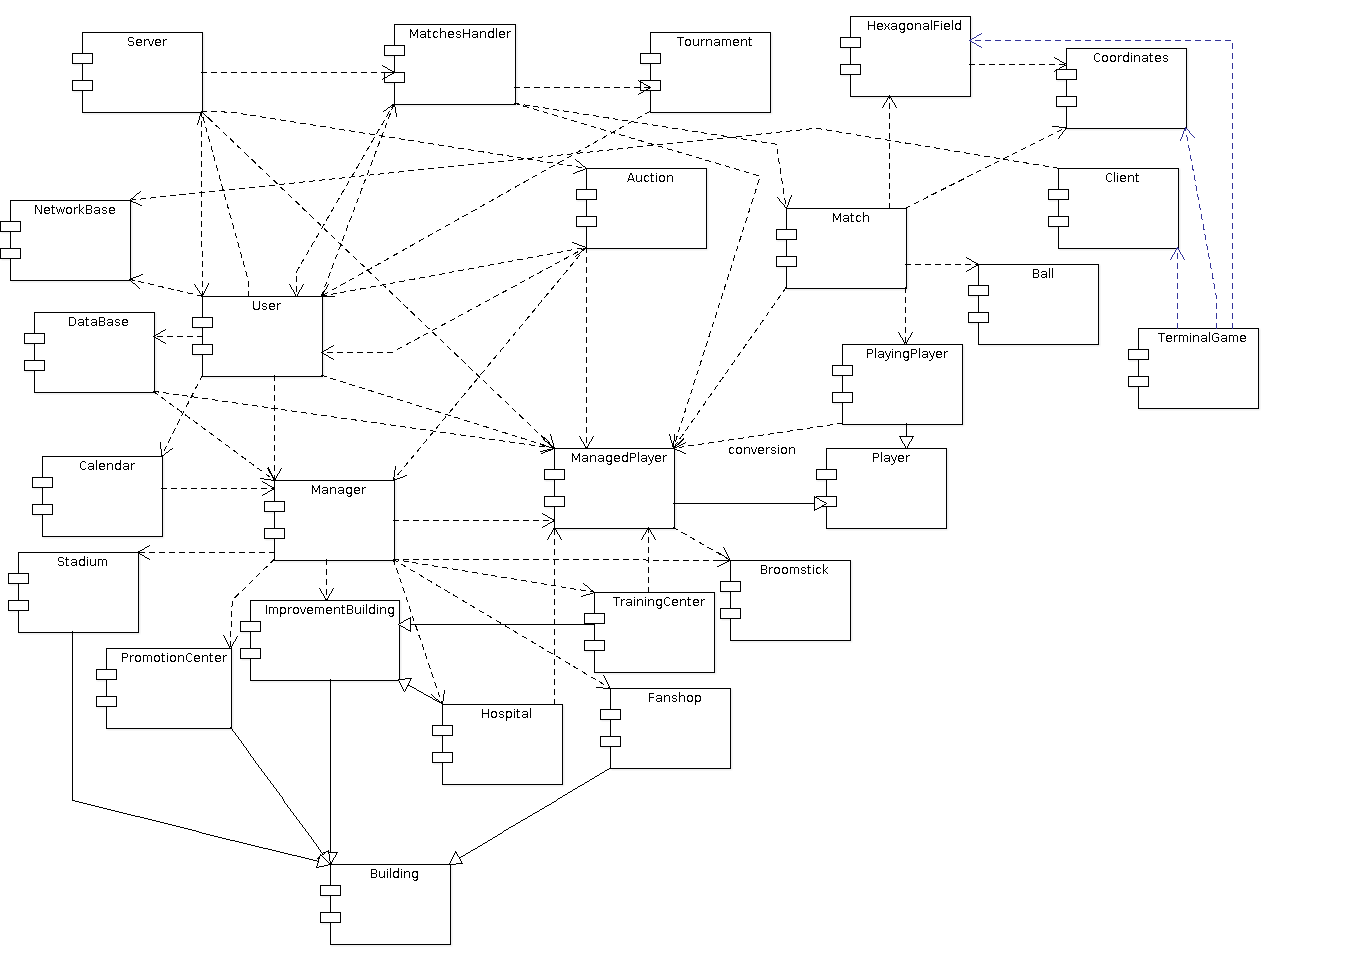
\includegraphics[scale=0.4]{uml/Diagrammededeploiement.png}
    \caption{Diagramme de composants}
    \end{figure}
    Lors de la phase suivante, nous veillerons à dissocier le client (réseau) de la gestion des affichages et entrées clavier du jeu en terminal.
    \begin{figure}[H]
    \center
    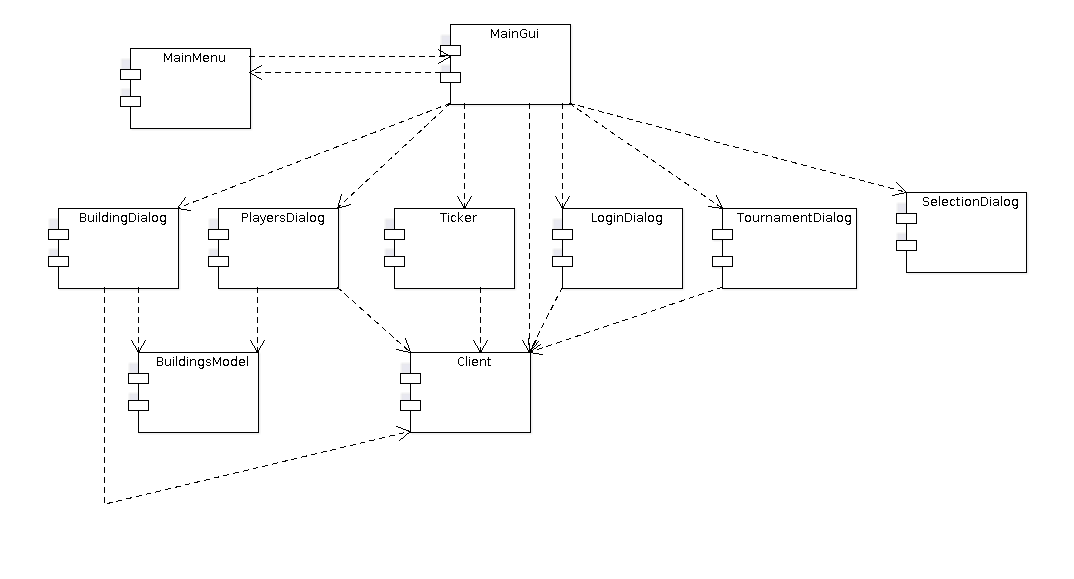
\includegraphics[scale=0.4]{uml/GUIComponents.png}
    \caption{Diagramme simplifié de composants pour la partie graphique uniquement}
    \end{figure}
\newpage

\section{Le client graphique} \label{diag-client-graphique}
\subsection{Le login}
Le client graphique s'ouvre sur un dialogue de login permettant à l'utilisateur de se connecter au serveur,
soit avec un nom d'utilisateur existant, soit en se créant une nouvelle identité \emph{(checkbox "New User")}\footnote{Les détails techniques de mise en \oe uvre sont mis entre parenthèses.
Un mode d'emploi s'obtiendra en supprimant ces parties.}.
A ce moment, la fenêtre du jeu n'est pas encore visible.\\
Si l'utilisateur ne souhaite pas se connecter ("Quit"), il se voit proposer une fenêtre avec
des menus réduits : "File" lui permettant de tenter à nouveau de se connecter ou, au contraire,
d'arrêter le programme, ainsi qu'un menu "Help".

\subsection{Les menus et les boutons}
En cas de réussite du login ou de l'enregistrement, le serveur fournit au client le rôle
de l'utilisateur : manager ou administrateur; ce dernier est réservé à l'utilisateur
"admin" (mode de passe "admin") prédéfini dans le fichier central d'identification.\\
En fonction de ce rôle, la fenêtre centrale de gestion \emph{(classe "MainGui" héritant de QMainWindow
: figure \ref{mainGUI})},
présente une barre de menus différente.\\
Le manager dispose également de boutons
\emph{(classe "MainMenu")} activant les fonctions associées aux points principaux de la barre de menus.
Ce rôle déterminera également de façon dynamique l'affichage de certains boutons dans le dialogue
de gestion des tournois.
    \begin{figure}[H]
    \center
    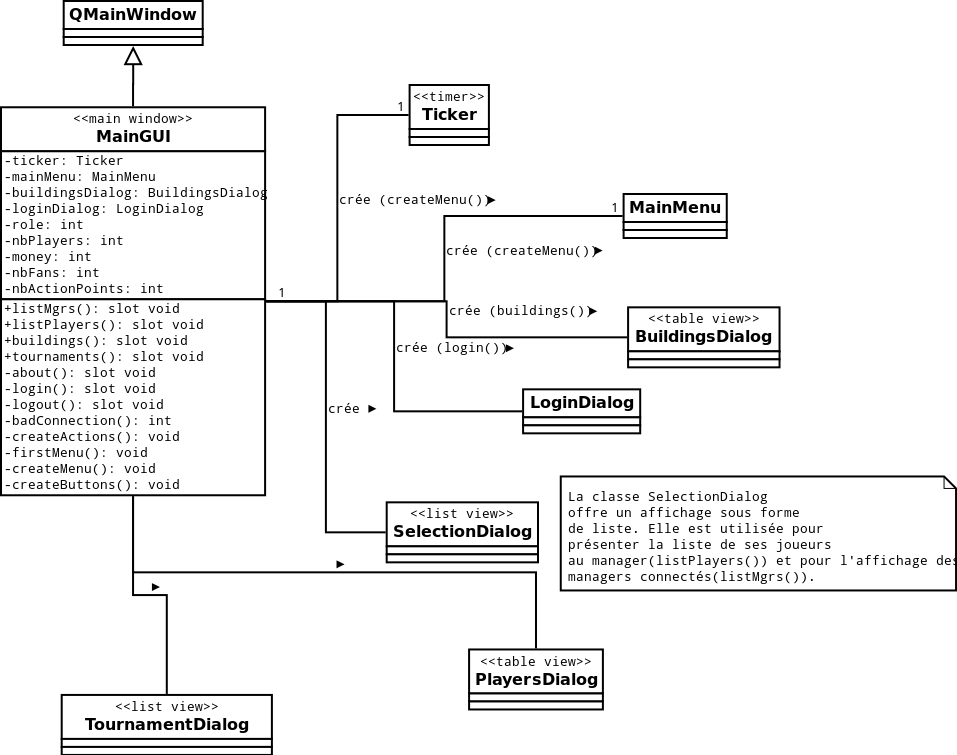
\includegraphics[scale=0.4]{uml/class/mainGUI.png}
    \caption{Diagramme de classes autour de "MainGui"} \label{mainGUI}
    \end{figure}
\subsection{La bannière}
Enfin, le manager voit s'afficher une bannière qui reprend les informations concernant ses avoirs;
ces informations sont rafraîchies périodiquement
\emph{(classe "ticker", qui, lorsqu'elle est affichée, lance un timer\cite{Blanchette2006})}.
L'utilisateur attentif remarquera que cette bannière se déplace : ce n'est pas un gadget;
à chaque déplacement, les données sont mises à jour!
\emph{(le but est, pour les développeurs, de pouvoir vérifier ainsi aisément que le timer fonctionne).}\\
Dans certaines parties du jeu, la bannière, moins utile, est cachée à dessein.
    \begin{figure}[H]
    \center
    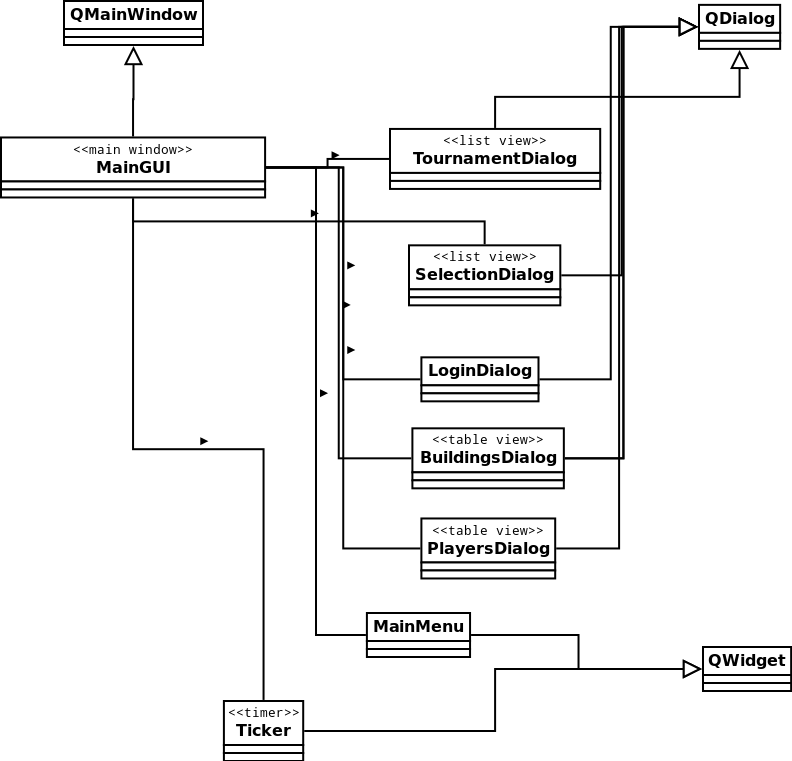
\includegraphics[scale=0.4]{uml/class/generalGUI.png}
    \caption{Diagramme de classes GUI} \label{generalGUI}
    \end{figure}
\emph{Comme le montre la figure \ref{generalGUI}, la majorité des classes graphiques héritent de "QDialog",
qui elle-même hérite de "QWidget", tout comme "QMainWindow".}

\subsection{La gestion des bâtiments}
Sous la forme d'un tableau de bord rafraîchi périodiquement \emph{(classe "BuildingsDialog")},
chaque ligne reprend l'état d'un bâtiment \emph{(une construction model-viewer
où le modèle "BuildingsModel", héritant de la classe abstraite "QAbstractTableModel", a été en partie réimplémenté;
un "reset()" avertit le viewer standard "QTableView" lorsque les données sont rafraîchies;
le modèle a été conçu pour être réutilisé, ce qui est le cas dans la gestion des joueurs : figure \ref{tableView})}.
    \begin{figure}[H]
    \center
    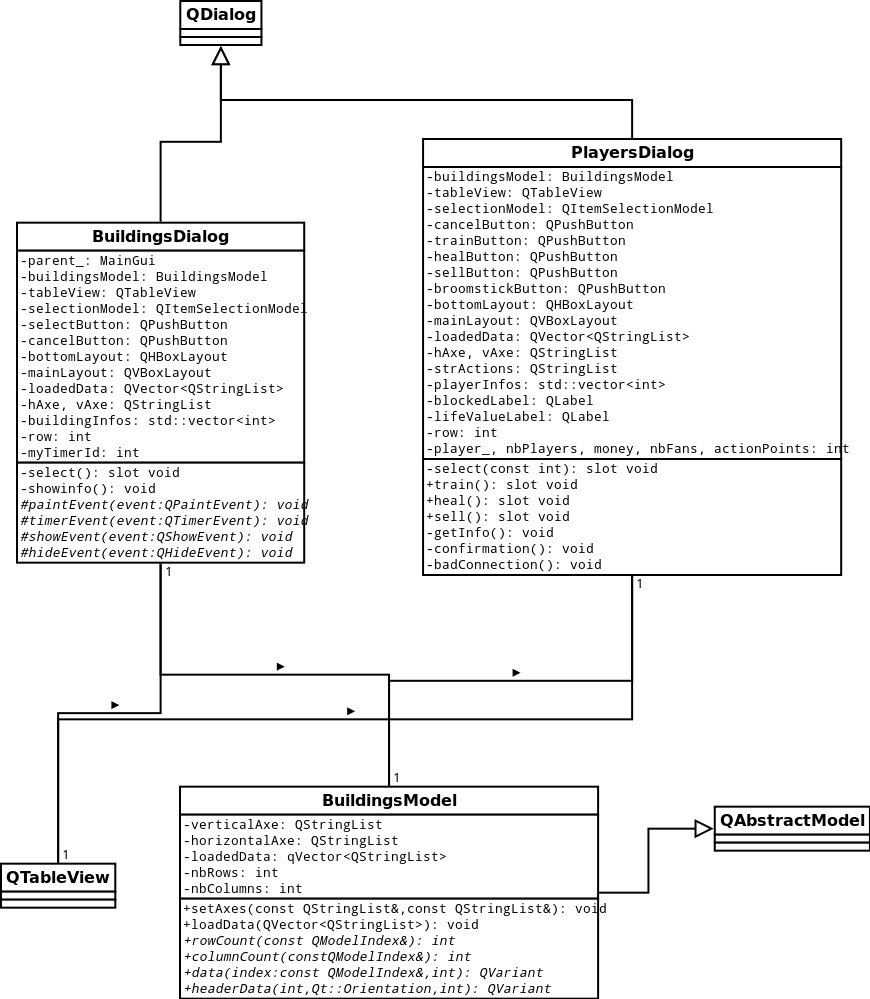
\includegraphics[scale=0.4]{uml/class/tableView.png}
    \caption{Diagramme des classes utilisant le modèle "BuildingsModel" associé au viewer "QTableView"}\label{tableView}
    \end{figure}
Le manager a la possibilité de demander un upgrade du bâtiment sur la ligne duquel
il a placé le curseur, si, bien entendu, il possède assez d'argent et de points d'action,
et que le bâtiment n'est pas déjà en cours d'upgrade.
Le manager peut entreprendre, à ces conditions, l'upgrade de plusieurs bâtiments.
S'il a la patience d'attendre la fin de ceux-ci, il verra,
sans devoir intervenir, les données du tableau de bord s'actualiser.
\subsection{La gestion des joueurs}
Cette fonction \emph{("playerMgr()")} commence par la présentation d'une liste
\emph{(une construction model-viewer autour d'une liste, placée dans une classe générique "SelectionDialog",
qui est réutilisée dans plusieurs autres fonctions)}
dans laquelle le manager peut sélectionner un joueur.
Cette présentation est un standard de l'application, repris dans toutes les fonctions;
elle permet de limiter au maximum le nombre d'entrées dans les menus,
car une fois le joueur sélectionné,
le programme lui présente les informations détaillées concernant ce dernier
et propose diverses actions sous forme de boutons,
en fonction des caractéristiques du joueur sélectionné.
Nous appellerons par la suite ce dispositif un modèle liste-détails-actions.\\
Les informations détaillées concernant le joueur sont ici à nouveau présentées sous la forme
d'un tableau de bord et d'une bannière \emph{(QLabel)}, en légende cette fois.
Si le joueur n'est pas bloqué car en cours d'entraînement, de soins ou de vente,
et que le manager dispose d'action points,
ce dernier voit apparaître des boutons lui permettant de lancer un entraînement, une vente
ou d'envoyer le joueur se faire soigner.
Bien entendu, ces boutons ne sont affichés que s'ils sont pertinents
par rapport à la situation présente du joueur.\\
Comme le manager ne peut entreprendre qu'une action à la fois,
le joueur étant alors bloqué pour un certain temps, la fonction s'arrête ensuite
\emph{(Ce dialogue est géré par la classe "playersDialog", qui, pour le tableau de bord,
met à nouveau en \oe uvre une construction model-viewer autour de la classe "BuildingsModel")}.
Notons que l'achat d'un broomstick est prévu mais pas encore programmé.
\subsection{Les tournois}
Cette fonction \emph{("tournaments()")} commence par un avertissement;
ensuite, comme pour la gestion des joueurs, vient la présentation d'une liste 
\emph{(une construction model-viewer gérée par la classe "SelectionDialog")}
dans laquelle le manager peut sélectionner un tournoi pour y participer,
si la liste n'est pas vide; sinon, il ne peut que quitter le dialogue.\\
Par contre, si l'utilisateur est un administrateur, il peut créer un nouveau tournoi
\emph{(Comme le nombre de données à introduire est limité,
nous avons eu recours ici, comme pour la vente d'un joueur, à une suite de questions,
plutôt qu'à la construction d'une classe adhoc héritant de "QDialog")}.

\section{Fonctionnalités futures envisagées}
  \subsection{Log des actions au cours d'un match}
    Lors de la gestion des déplacements au cours d'un match, le serveur enregistrerait 
    toutes les actions intervenues (collisions, tentative d'attraper le vif d'or,...).
    Il enverrait ce détail au client qui l'afficherait. Ainsi l'utilisateur aurait une
    meilleure compréhension de ce qui se déroule entre deux tours.
  \subsection{Ajouter des possibilités à l'administrateur}
    L'administrateur disposerait d'un plus large panel d'options, dont par exemple :
    \begin{itemize}
      \item Bannir, bloquer, ou supprimer un compte utilisateur.
      \item La création d'un compte utilisateur avec des caractéristiques de départ choisies.
      \item La possibilité de créer un joueur avec des caractéristiques choisies 
        et de l'attribuer à un utilisateur ou de le mettre aux enchères.
      \item La possibilité de récupérer les données du serveur afin d'en faire une sauvegarde locale.
    \end{itemize}
  \subsection{Des matchs d’entraînement}
    À l'aide d'une intelligence artificielle basique, permettre à l'utilisateur
    de jouer un match d'entraînement, ne rapportant pas d'argent mais
    augmentant les capacités des joueurs en fonction de leurs succès.
    
  


%\chapter{Index des termes utilisés}
%  Contiendra, au moins, toutes les entrées du glossaire (avec les numéros des pages correspondantes).
\addcontentsline{toc}{chapter}{4 Index}
\phantomsection
\begin{thebibliography}{9}
\bibitem{Blanchette2006} Blanchette Jasmin, Summerfield Mark - Trolltech 2006 - C++ GUI programming with Qt4 - ISBN 0-13-187249-4
\bibitem{Bulfone} Bulfone Christian - 2012 - Le modèle client-serveur - www.gipsa-lab.fr/~christian.bulfone/IC2A-DCISS
\end{thebibliography}
\printindex

\end{document}
